\chapter{Neue Auswahlkomponente}
\label{chap:newComponent}

Dieses Kapitel beschreibt die Bausteine der neuen Komponente auf verschiedenen Ebenen. 
Als Erstes zeigt das Design die visuellen Darstellungsmöglichkeiten über die getroffene Auswahl bis hin zu den Prototypen. 
Dazu gesellen sich sowohl die Implementation der Zustände als auch die Umsetzung des Designs.
Darauffolgend findet sich die Definition der Interaktion mit der Maus wie auch der Tastatur. 
Die für einen stabilen Code wichtigen Regeln und Prinzipien sind ebenfalls festgelegt. 
Die Anwendung diverser Patterns führt zu einer klaren Struktur und hoher Wiederverwendbarkeit. 
Als spezielles Element in der View zählt der Dropdown-Container. 
Dieser lässt sich unterschiedlich implementieren. 
Für ein angenehmes Nutzerfeeling spielt eine gute Performance eine tragende Rolle. 
Dies zeigen auch die ausgeführten User-Tests mit Endanwendern wie auch Programmierern. 
Automatisierte Tests für jede Komponente beweisen eine gute Codequalität. 


\section{Design}
\label{sec:design}

Das Ziel ist, eine konsistente und ansprechende Benutzererfahrung zu schaffen, die sich über alle modernen Browser hinweg hält. 
Das Design der neuen Auswahlkomponente ist stark vom Kolibri-Designsystem inspiriert. 
Das Designsystem bietet bereits ein umfassendes Set von Richtlinien und Komponenten. 
Diese ermöglichen eine einheitliche und benutzerfreundliche Gestaltung von Anwendungen. 
Das neue Design enthält jedoch einige Anpassungen, um die Lesbarkeit zu optimieren. 
Dazu benötigt es eine Analyse der Möglichkeiten, welche im nachfolgenden Kapitel beschrieben sind. 


\subsection{Mögliche Designoptionen eines Elements \& deren Wahl}
\label{sec:possibleDesignOptions}

Elemente lassen sich durch diverse Eigenschaften stylen. 
Die Anpassung der Hintergrundfarbe fällt am schnellsten ins Auge. 
Diese ist hell zu gestalten, damit der Kontrast zur dunklen Default-Schriftfarbe erhalten bleibt. 
Der Rahmen bietet eine weitere Designmöglichkeit. 
Seine Farbe, Dicke oder Struktur können variieren. 
Eine andere Alternative ist, nur eine Seite des Rahmens zu verwenden. 
Als Beispiel dafür gilt der sogenannte Spiegelstrich, welcher auf der linken Seite platziert ist. 
Für eine gute Erkennbarkeit sollte die Färbung rund um den Rahmen in einer eher dunklen Schattierung Anwendung finden. 
Als weitere Style-Eigenschaften bieten sich Änderungen der Schrift an. 
Bei der Farbe ist der Kontrast zu beachten, weswegen eine eher dunkle zu wählen ist. 
Alternativ lassen sich die Dicke, Schriftart, Neigung, Grösse oder Dekoration ändern. 
All diese Style-Anpassungen lassen sich auf unterschiedliche Art und Weise kombinieren. 

Bei den Farben existiert eine grosse Bandbreite. 
Da Kolibri bereits ein Designsystem besitzt, schränkt sich die Menge ein. 
Unter den vorhandenen Farbwerten bieten sich die Folgenden am besten an: 

\begin{itemize}
    \item Kolibri-Light/Yellow/100 $\rightarrow$ helles Weiss-Gelb
    \item Kolibri-Light/Yellow/300 (\codestyle{-{}-kb-color-select}) $\rightarrow$ helles Gelb
    \item Kolibri-Light/Warning/\codestyle{-{}-kb-warning-dark} $\rightarrow$ dunkles Gelb
    \item Kolibri-Light/Danger/\codestyle{-{}-kb-danger-accent} (\codestyle{-{}-kolibri-color-accent}) $\rightarrow$ mittleres Rosa
    \item Kolibri-Light/Success/\codestyle{-{}-kb-success-accent} $\rightarrow$ mittleres Grün
    \item Kolibri-Light/Success/\codestyle{-{}-kb-success-light} $\rightarrow$ helles Grün
    \item Kolibri-Light/Primary/\codestyle{-{}-kb-primary-accent} $\rightarrow$ mittleres Violett
    \item Kolibri-Light/Primary/\codestyle{-{}-kb-primary-light} $\rightarrow$ helles Violett
    \item Kolibri-Light/Secondary/\codestyle{-{}-kb-secondary-accent} $\rightarrow$ mittleres Blau
    \item Kolibri-Light/Secondary/\codestyle{-{}-kb-secondary-light} $\rightarrow$ helles Blau
    \item Kolibri-Light/Monochrome/\codestyle{-{}-kb-color-body} $\rightarrow$ mittleres Grau
    \item Kolibri-Light/Monochrome/\codestyle{-{}-kb-color-line} $\rightarrow$ helles Grau
\end{itemize}

Da die Elemente drei verschiedene Zustände gleichzeitig erhalten können, müssen die Styles kombinierbar sein. 
Nicht jede der erwähnten Eigenschaften und Farben eignet sich in gleichem Masse. 
\emph{Yellow-100} fällt schnell wieder weg, da je nach Display der Kontrast zu gering ist. 
Unter den restlichen hellen Schattierungen passt \emph{Yellow-300} am besten. 
Diese Farbe ist bereits als Selektionsfarbe im Code hinterlegt. 
Als Hintergrundfarbe eignet sich am ehesten das vordefinierte \codestyle{-{}-kb-color-select}. 
Dadurch ist klar, dass die anderen beiden Zustände eine eher kräftige bzw. dunkle Färbung benötigen. 
Der Blick auf die Namen im Designsystem zeigt eine weitere Farbe zur Hervorhebung eines Elements. 
Die Benennung des mittleren Rosas mit Accent (\codestyle{-{}-kolibri-color-accent}) bietet einen guten Kontrast zur Selektion. 
Diese Farbe ist ebenfalls im Code vordefiniert. 
Da die dritte Farbe nicht zu viel Unruhe in das Design bringen soll, schränkt sich die Farbauswahl weiter ein. 
Mit einem gut erkennbaren Kontrast zur Selektion bietet sich das dunkle Gelb \codestyle{-{}-kb-warning-dark} an. 

Wie erwähnt ist die Eigenschaft Hintergrundfarbe durch die Wahl der Farbe bereits festgelegt. 
Die Änderung der Schrift sollte maximal die Farbe betreffen. 
Die anderen Font-Stylings sind schwer erkennbar oder zerstören das Bild. 
Der komplette Rahmen passt nicht in das Design und fällt somit ebenfalls weg. 
Da nicht beide Zustände auf die Schriftfarbe zugreifen können, bietet sich der oben genannte Spiegelstrich an. 
Das Rosa mit einem guten Kontrast zum Gelb findet sich im linksseitigen Rahmen wieder. 
Das dunkle Gelb färbt – nebst dem linksseitigen Strich – die Schrift. 
Die Zuordnung der Designwahl zu den fehlenden Zuständen steht im Kapitel \textbf{\nameref{sec:colorContrast}}. 


\clearpage
\subsection{Figma-Prototypen}
\label{sec:figmaPrototype}

Zur Visualisierung und zum interaktiven Testing des Designs kommt Figma zum Einsatz. 
Figma ist ein webbasiertes Tool zur Erstellung von UI/UX-Designs, das Echtzeit-Kollaboration ermöglicht. 
Das Sammeln der Feedbacks von Stakeholdern und Nutzern unterstützt eine effiziente Entwicklung. 
Dafür ist es unabdingbar, im Vorfeld mit Figma schnell Prototypen zu erstellen und mit den Probanden zu teilen. 
Das Arbeiten mit Figma-Komponenten erleichtert das Entwickeln enorm. 
Dies ermöglicht das Erstellen von Varianten ohne viel Aufwand. 

Die folgenden Screenshots \ref{img:figmaPrototype1} bis \ref{img:figmaPrototype3} zeigen die Prototypen der neuen Drop\-down-Kom\-po\-nente. 

\begin{figure}[!htb]
    \centering
    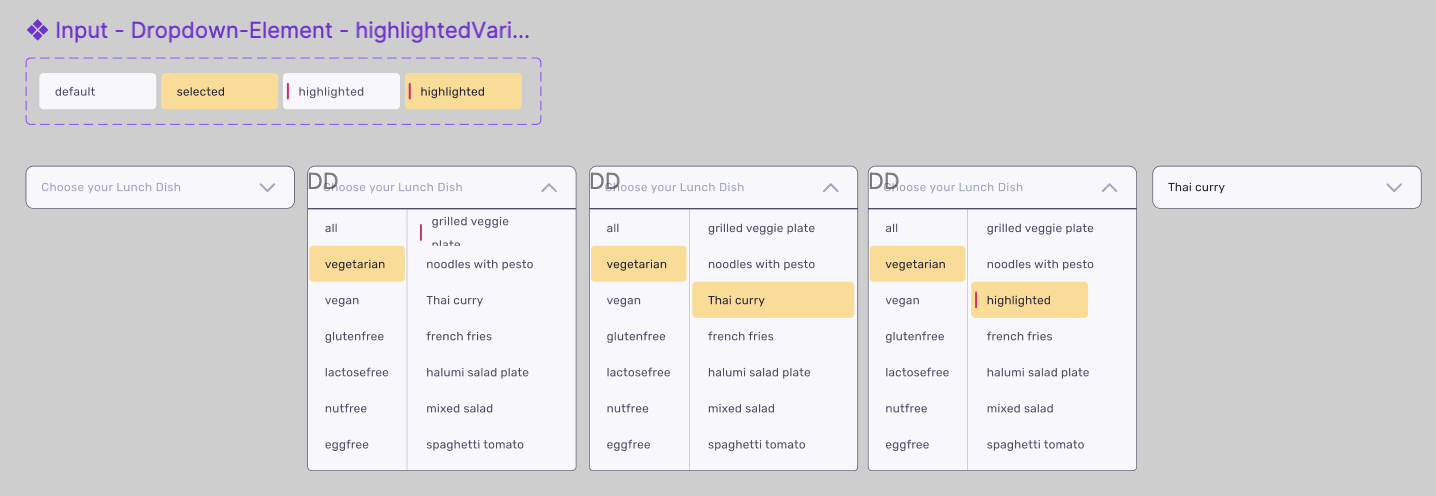
\includegraphics[width=100mm]{figma-prototype-1.png}
    \caption{\centering Neue Komponente – Menüauswahl}
    \label{img:figmaPrototype1}
\end{figure}

\begin{figure}[!htb]
    \centering
    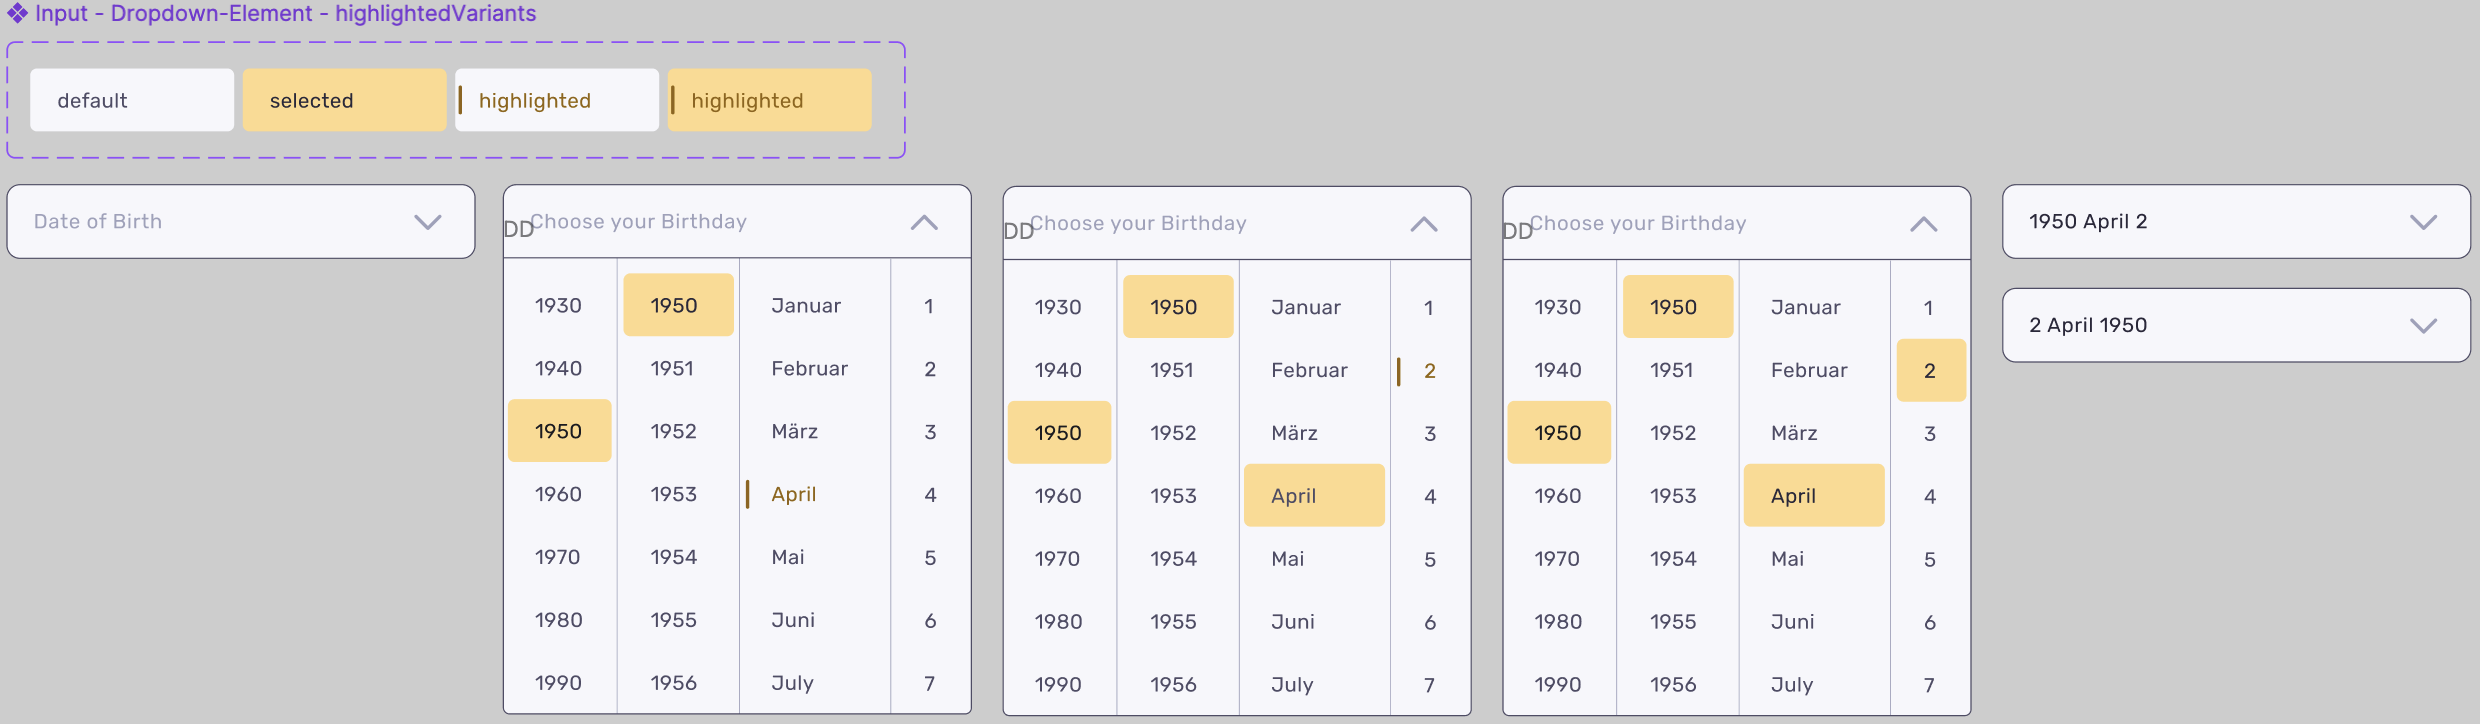
\includegraphics[width=100mm]{figma-prototype-2.png}
    \caption{\centering Neue Komponente – Geburtstag}
    \label{img:figmaPrototype2}
\end{figure}

\begin{figure}[!htb]
    \centering
    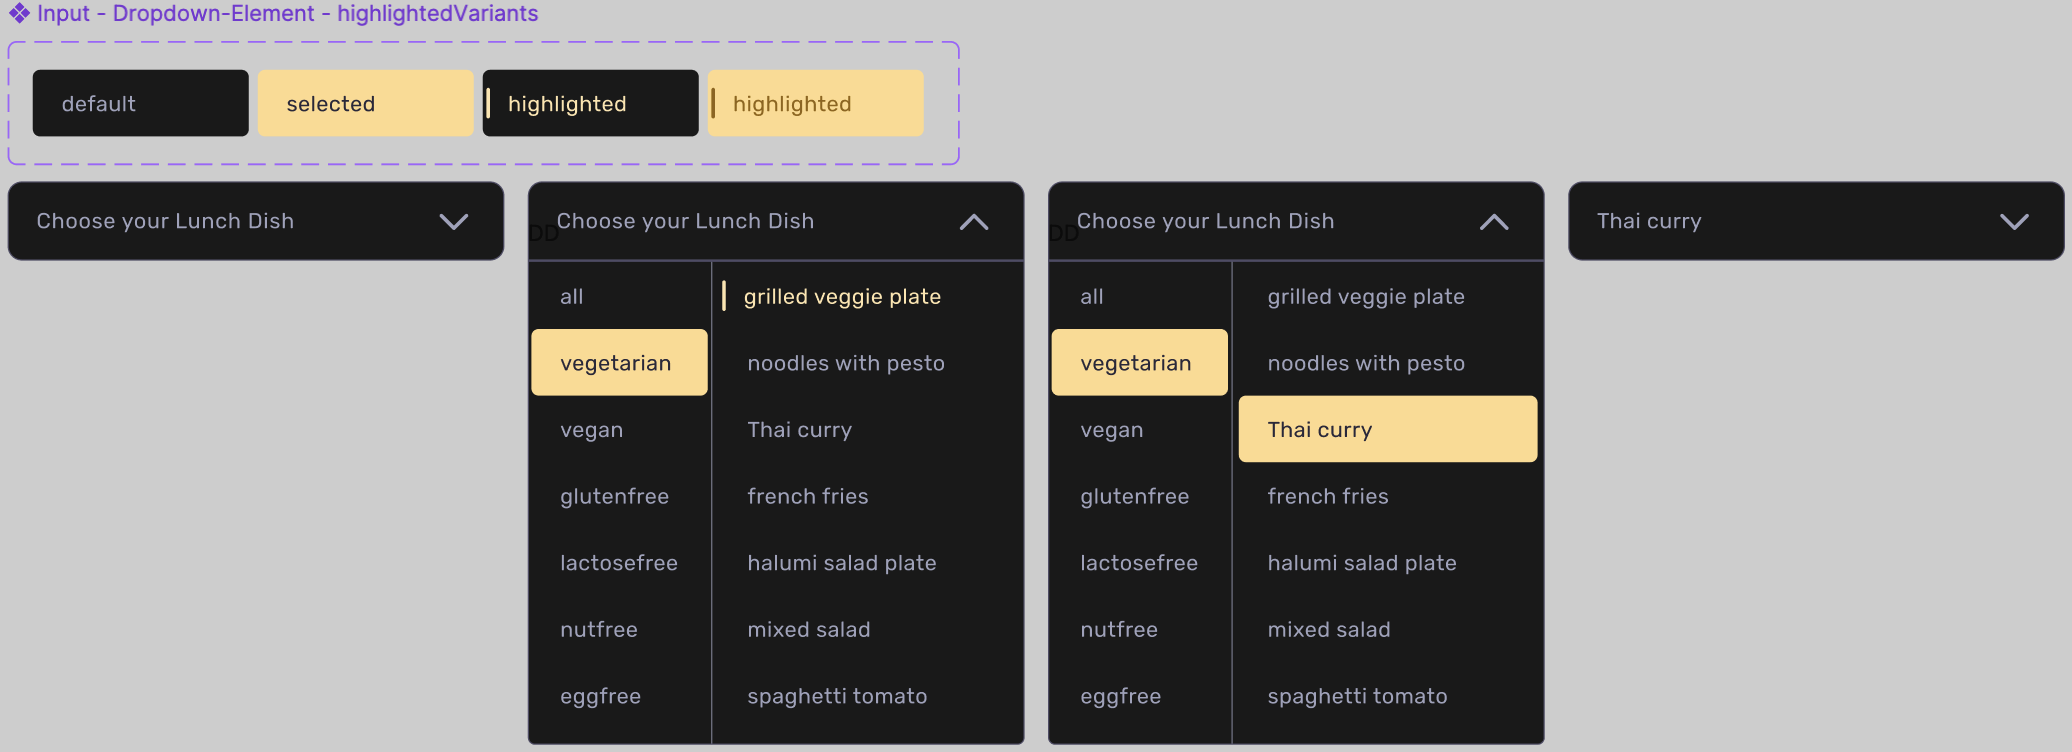
\includegraphics[width=100mm]{figma-prototype-3.png}
    \caption{\centering Neue Komponente im Dark-Mode}
    \label{img:figmaPrototype3}
\end{figure}

Die ersten beiden Grafiken bilden die Komponente in verschiedenen Anwendungsgebieten ab. 
Die Abbildung \ref{img:figmaPrototype3} zeigt ein mögliches Design für einen Dark-Mode. 
Dabei sind die Farben so weit angepasst, dass der Kontrast weiterhin gegeben ist. 


\subsection{Farbpalette}
\label{sec:colorContrast}

Das Kolibri-Designsystem bietet eine Vielzahl von Farben. 
Der Figma-Prototyp enthält spezifische Anpassungen, so dass die Dropdown-Komponente gut lesbar ist. 
Für den Erhalt einer besseren Nutzerfreundlichkeit gestaltet sich die Farbauswahl aus Abbildung \ref{img:designColors}. 

\begin{figure}[!htb]
    \centering
    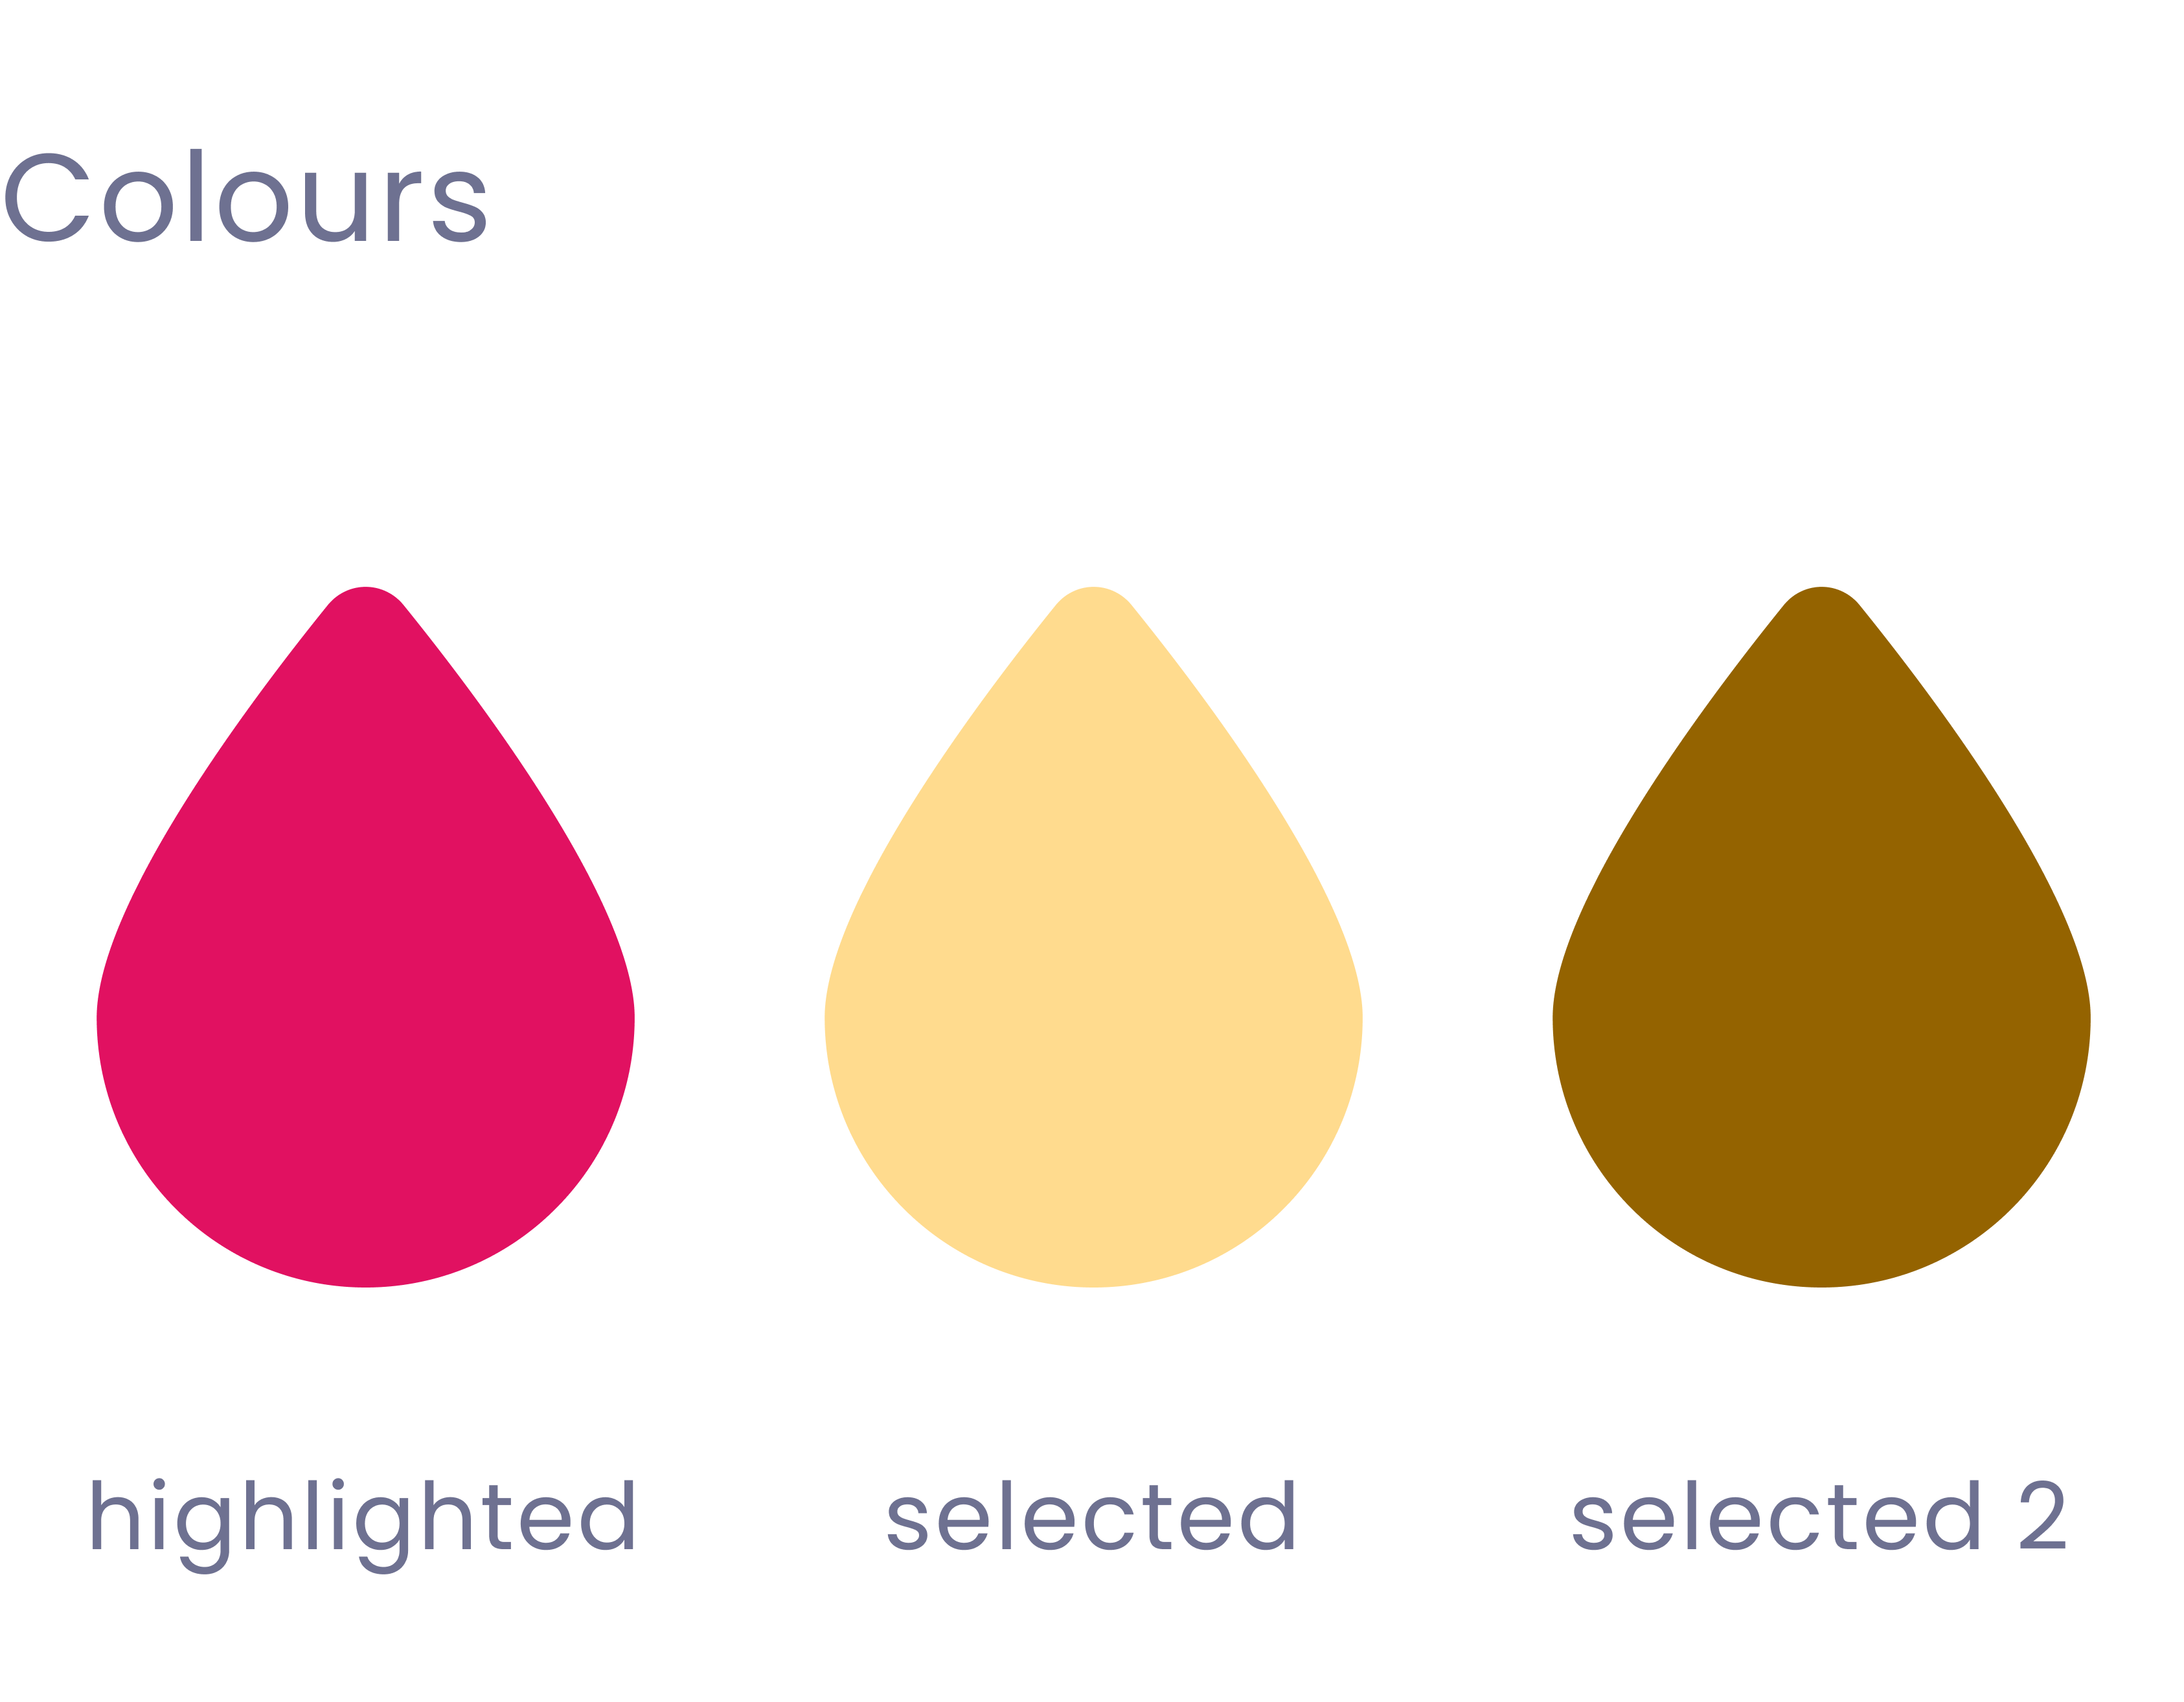
\includegraphics[width=70mm]{design-colors.png}
    \caption{\centering Farbpalette der neuen Komponente}
    \label{img:designColors}
\end{figure}

Diese bietet hohen Kontrast und verbessert somit die Barrierefreiheit der Anwendung. 
Die Gründe der Auswahl befinden sich im früheren Kapitel \textbf{\nameref{sec:possibleDesignOptions}}. 
Die Zustände verbinden sich wie folgt mit der getroffenen Wahl der Farben. 

\begin{itemize}
    \item \textbf{Original} $\rightarrow$ \textbf{Neu}
    \item Kolibri-Light/Yellow/300 $\rightarrow$ selected
    \item Kolibri-Light/Danger/\codestyle{-{}-kb-danger-accent} $\rightarrow$ highlighted
    \item Kolibri-Light/Warning/\codestyle{-{}-kb-warning-dark} $\rightarrow$ cursor position
\end{itemize}

Bei der Verwendung dieser Farben in der neuen Komponente sind einige CSS-Dateien notwendig. 
Diese dienen als Grundlage für das weitere Design. 
Der Code \ref{code:cssImports} zeigt die importierten CSS-Files. 

\begin{lstlisting}[style = htmlcssjs, caption = Notwendige CSS-Imports, label = code:cssImports]
@import "../../../css/kolibri-base.css";
@import "../../../css/kolibri-light-colors.css";
\end{lstlisting}

Die erste Zeile enthält die grundlegenden Kolibri Designs. 
Dazu gehören einige vordefinierte Farben wie eine Selektion oder ein Highlight. 
Weiterhin sind die Schriften und die Invalidität von Inputs festgelegt. 
Die zweite Datei ist für die breite Palette an Farben im Light-Mode zuständig. 


\subsection{Layout und Animation}
\label{sec:layoutTypo}

Die Dropdown-Komponente besteht aus der Detail- und der Master-Ansicht. 
Dieser Aufbau ist im Kapitel \textbf{\nameref{sec:masterDetailView}} genauer beschrieben. 
Das Layout innerhalb des Option-Popovers liegt in Spalten vor. 
Die einzelnen Optionen listen sich zeilenweise in den Spalten auf. 
Der Listencontainer öffnet sich mit einer Animation. 
Nachfolgender Codeausschnitt \ref{code:popoverStyle} zeigt die dafür relevanten Zeilen. 

\begin{lstlisting}[style = htmlcssjs, caption = Animation zum Öffnen des Popovers, label = code:popoverStyle]
/* animation */
@keyframes open {
    0%   { transform: scaleY(0); }
    100% { transform: scaleY(1); }
}
/* popover closed */
[popover] {
    display:          none;
    animation:        open 300ms ease-in-out;
    transform-origin: top center;
}
@starting-style {
    [popover]:popover-open {
        height:       0;
    }
}
/* popover opened */
[popover]:popover-open {
    display:          flex;
    height:           fit-content;
}
\end{lstlisting}

Die grundlegenden Styling-Properties des Popover-Containers sind nicht aufgeführt. 
Die CSS-Regeln aus Code \ref{code:popoverStyle} definieren die öffnende Animation des Popovers. 
Das \codestyle{@keyframes} regelt die Transformation bzw. Animation, welche das Ausfahren des Containers festlegt. 
Das \codestyle{[popover]} steuert das Erscheinungsbild des geschlossenen Popovers. 
Die Animation ist mit Zeile 9 an den Popover-Container gebunden. 
Die Zeilen 12 bis 16 definieren die CSS-Regeln, welche zum Start des Öffnens gelten. 
Der Selektor \codestyle{:popover-open} legt die Darstellung des offenen Zustands fest. 

Das Togglen des Popover erhält zusätzlichen Code, damit der Controller aktuell bleibt. 
Das entsprechende Event aus Codeausschnitt \ref{code:popoverToggle} führt ein Update auf dem Controller aus. 

\begin{lstlisting}[style = htmlcssjs, caption = Event-Handling für Popover-Toggle, label = code:popoverToggle]
optionsContainer.addEventListener("toggle", (event) => {
    if (event.newState === "open") {
        optionsContainer.classList.toggle("opened", true);
        selectController.setOptionsVisibility(true);
    } else {
        optionsContainer.classList.toggle("opened", false);
        selectController.setOptionsVisibility(false);
    }
    // more code to update scrollbars in columns
});
\end{lstlisting}

Dieser Code (\ref{code:popoverToggle}) prüft beim Togglen den neuen Status des Events. 
Anhand des Status erhält das Popover ein Update bei den Klassen. 
Die weiteren Zustände sind im nachfolgenden Kapitel genauer beschrieben. 


\subsection{Implementation der Zustände}
\label{sec:implementStates}

Die Auswahlkomponente ist so gestaltet, dass sie sowohl für Maus- als auch Tastaturbenutzer optimal funktioniert. 
Das Design der Interaktionen bietet eine intuitive und leicht zugängliche Bedienung der Komponente. 
Spezifische CSS-Klassen erleichtern die Benutzerführung. 
Sie definieren die Styles der hervorgehobenen (highlighted) bzw. ausgewählten (selected) Optionen. 
Die Cursor-Position erhält ebenfalls eine eigene CSS-Klasse. 
Dieser Zustand wie auch das Highlight sind unter anderem durch einen Spiegelstrich dargestellt. 
Der CSS-Code \ref{code:styledElement} zeigt einen Style-Ausschnitt auf ein Cursor-Position-Element. 

\begin{lstlisting}[style = htmlcssjs, caption = Spiegelstrich der Cursor-Position, label = code:styledElement]
.cursor-position::before {
    content:       '';
    position:      absolute;
    left:          7px;
    top:           0.5em;
    bottom:        0.4em;
    transform:     translateX(-50%);

    background:    var(-{}-kb-hsla-warning-dark);
    border-radius: 1px;
    width:         2px;
}
\end{lstlisting}

Der Selektor \codestyle{.cursor-position} befindet sich immer nur auf einem Element – der Cursor-Position. 
Die Zeilen 2 bis 6 in Code \ref{code:styledElement} definieren die Position des Spiegelstrichs. 
Das Erscheinungsbild ist durch die Zeilen 8 bis 10 beschrieben. 
Eine dunkle Farbe und eine linksseitige Markierung betonen das Element der Cursor-Position. 
Das Highlight verwendet einen sehr ähnlichen Code. 
Die Farbe wie auch die Position sind jedoch angepasst. 
Zudem hält sich das Highlight nicht an eine Klasse, sondern nutzt die Pseudo-Klasse \codestyle{:hover}. 

Für ein konsistent gehaltenes UI sind diverse Event-Handler und UI-Update-Funk\-tion\-en notwendig. 
Im \codestyle{columnOptionsProjector.js} existiert beispielsweise ein Event-Hand\-ler. 
Er steuert das Setzen und Entfernen der Selektionsklasse. 
Dieser ist im nachfolgenden Code \ref{code:selectionChange} ersichtlich. 

\begin{lstlisting}[style = htmlcssjs, caption = Änderung der Selektion, label = code:selectionChange]
const selectOptionItem = (root) => (newOption, oldOption) => {
    const oldItem = getHtmlElementByOption(oldOption, root);
    if (oldItem) {
        oldItem.classList.remove("selected");
    }

    const newItem = getHtmlElementByOption(newOption, root);
    if (newItem) {
        newItem.classList.add("selected");
    }
}; 
\end{lstlisting}

Die Funktion \codestyle{selectOptionItem} verschiebt die Klasse \codestyle{selected} vom Alten auf das neue Element. 
Dadurch passt sich das UI automatisch an. 
Damit sich die Änderung nur auf die Selektion der aktuellen Spalte auswirkt, verlangt die Funktion ein Elternelement. 
Das hier versendete \codestyle{getHtmlElementByOption} sucht im Teilbaum des DOMs das HTML-Element zur mitgegebenen Option. 


\subsection{Prototyping}
\label{sec:userFeedbackPrototyping}

Der Einsatz von interaktiven Figma-Prototypen ist hilfreich beim Evaluieren der Benutzerfreundlichkeit und intuitiven Bedienung. 
Die Prototypen der neuen Auswahlkomponente bauen auf dem Resultat der Vorarbeit auf. 
Daher sind keine Low-Fi-Gestaltungen notwendig. 
Die Einbindung der in der Vorarbeit erhaltenen Feedbacks der Länderkomponente findet in den neuen Hi-Fi-Prototypen ihre Anwendung. 
Beispiele für die Designs sind in der Grafik \ref{img:figmaPrototype1} ersichtlich. 
Im oberen Bereich des Bildes befinden sich die Zustände der Optionen. 
Benutzertests decken die Mängel und Wünsche der Probanden auf. 
Mit der Integration der Rückmeldungen von Benutzerinteraktionen in das Design verbessert sich die Usability kontinuierlich. 
Mehr zu den Nutzerfeedbacks folgt im Kapitel \textbf{\nameref{sec:userTests}}. 
Das Resultat des umgesetzen Prototypen ist im nachfolgenden Kapitel genauer beschrieben. 


\subsection{Implementationsresultat}
\label{sec:designImplementation}

Die diversen oben beschriebenen Design-Schritte resultieren in den Abbildungen \ref{img:closedNewComponent} bis \ref{img:openedThreeColCatNewComponent}. 
Weitere Bilder befinden sich im Anhang \textbf{\ref{chap:newImgs}}. 

\begin{figure}[!htb]
    \centering
    \begin{minipage}[b]{0.3\textwidth}
        \centering
        \begin{minipage}[t]{\textwidth}
            \centering
            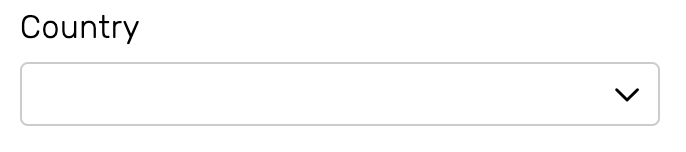
\includegraphics[width=\textwidth]{newComponent/closed.png}
            \caption{\centering Geschlossene \codestyle{SelectComponent}}
            \label{img:closedNewComponent}
        \end{minipage}
        \vspace{0.6cm}\newline
        \begin{minipage}[b]{\textwidth}
            \centering
            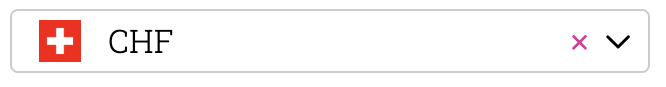
\includegraphics[width=\textwidth]{newComponent/closed.img.png}
            \caption{\centering Ausgefüllte \codestyle{SelectComponent}}
            \label{img:closedImgNewComponent}
        \end{minipage}
        \newline
    \end{minipage}
    \hfill
    \begin{minipage}[b]{0.35\textwidth}
        \centering
        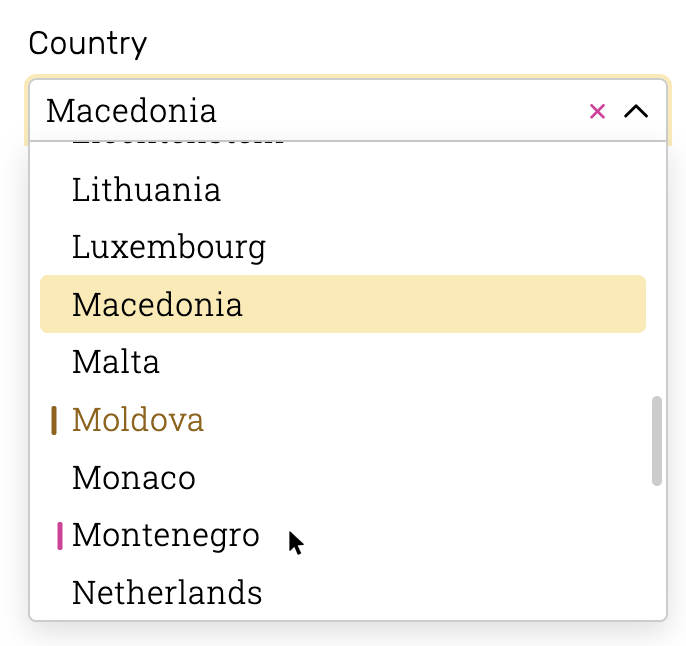
\includegraphics[width=0.9\textwidth]{newComponent/opened.selected.cursored.highlighted.png}
        \caption{\centering Offene \codestyle{SelectComponent} – 3 Zustände}
        \label{img:openedHighlightedCursoredSelectedNewComponent}
    \end{minipage}
    \hfill
    \begin{minipage}[b]{0.25\textwidth}
        \centering
        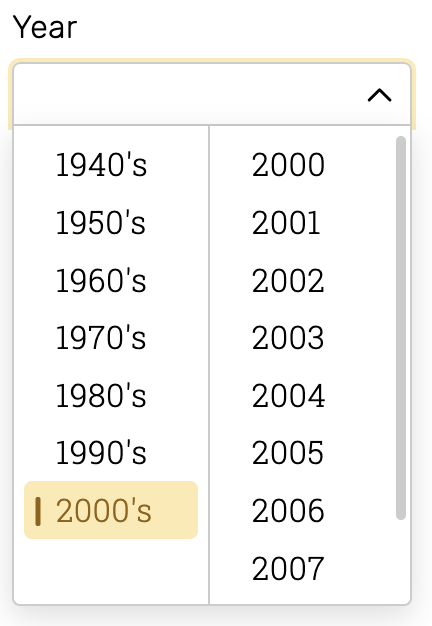
\includegraphics[width=0.8\textwidth]{newComponent/opened.2col.categoried.png}
        \caption{\centering Offene \codestyle{SelectComponent} – 2 Spalten}
        \label{img:openedTwoColCatNewComponent}
    \end{minipage}
\end{figure}

Im geschlossenen Zustand (Abbildungen \ref{img:closedNewComponent}) zeigt der Pfeil auf der rechten Seite nach unten. 
Das Icon ändert beim Öffnen der neuen Komponente die Richtung und zeigt nach oben (Abbildungen \ref{img:openedHighlightedCursoredSelectedNewComponent}). 
Die selektierte Option kann wie in der Grafik \ref{img:closedImgNewComponent} ein Bild enthalten. 
Der Fokus auf der \codestyle{SelectComponent} ist durch einen gelben Rahmen um die Detail-Ansicht visualisiert. 
Dies ist in Abbildung \ref{img:openedTwoColCatNewComponent} im oberen Bereich ersichtlich. 
Ist das Feld \codestyle{required}, erhält der Rahmen einen rosafarbenen Rahmen. 
Dabei ist der Fokus aber nicht überdeckt. 
Die \codestyle{disabled} \codestyle{SelectComponent} zeigt sich wie die anderen Eingabefelder ebenfalls ausgegraut. 

Die offene Komponente stellt den Options-Container in jedem Fall unterhalb dar. 
Die Abbildung \ref{img:openedHighlightedCursoredSelectedNewComponent} enthält – nebst Normal – die drei möglichen Zustände der einzelnen Optionen. 
Der Wert \emph{Macedonia} visualisiert die Selektion, welche sich ebenfalls im oberhalb befindlichen Detail-Container wiederfindet. 
\emph{Moldova} zeigt die Optionen mit der Cursor-Position und somit die Stelle, an welcher sich die Tastatur befindet. 
Das Highlight enthält den Wert \emph{Montenegro}. 
Die Cursor-Position und das Highlight können auf der gemeinsamen Option liegen. 
Dabei sind beide Zustände sichtbar. 

Die Abbildungen \ref{img:openedTwoColCatNewComponent} bis \ref{img:openedThreeColCatNewComponent} zeigen, dass die \codestyle{SelectComponent} mehrere Spalten besitzen kann. 

\begin{figure}[!htb]
    \begin{minipage}[b]{0.43\textwidth}
        \centering
        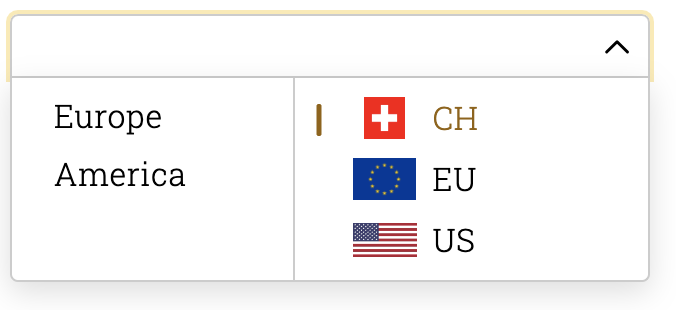
\includegraphics[width=0.9\textwidth]{newComponent/opened.img.png}
        \caption{\centering Offene \codestyle{SelectComponent} mit Bildern}
        \label{img:openedTwoColImgNewComponent}
    \end{minipage}
    \hfill
    \begin{minipage}[b]{0.47\textwidth}
        \centering
        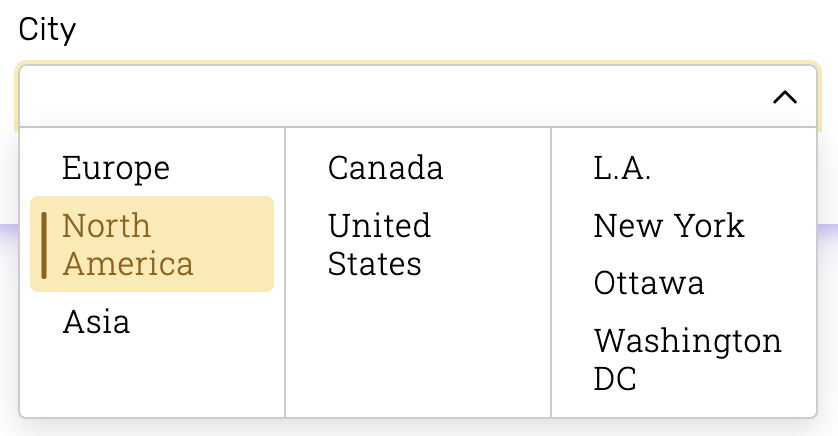
\includegraphics[width=0.8\textwidth]{newComponent/opened.3col.categoried.png}
        \caption{\centering Offene \codestyle{SelectComponent} – 3 Spalten}
        \label{img:openedThreeColCatNewComponent}
    \end{minipage}
\end{figure}

In diesen Beispielen befindet sich die Value-Option\footnote{
    Formular-Wert, wenn einer selektiert ist
} jeweils in der rechten Spalte. 
Die anderen Spalten dienen zur Filterung der Werte. 
Die Grafik \ref{img:openedTwoColImgNewComponent} mit der Selektion \emph{2000's} begrenzt die Jahreszahlen von ursprünglich 70 auf noch 10 Werte. 
Wenn mehrere Kategorien existieren, bewirkt eine Selektion ganz links eine Reduktion aller Optionen, die auf der rechten Seite liegen. 
In der Abbildung \ref{img:openedThreeColCatNewComponent} bewirkt die Wahl von \emph{North America} die Reduktion der Länder und der Städte. 


\section{Interaktionen}
\label{sec:interaction}

Damit ein gemeinsames Verständnis entsteht, gilt es für die Bedienung der Komponente Regeln festzulegen. 
Wie in den Grundlagen bereits beschrieben kann sich ein Wert aus dem Optionen-Container in verschiedenen Zuständen befinden. 
In diesem Absatz spielen Selektion, Highlight und Cursor-Position eine Rolle. 
Zur Auffrischung: 

\begin{itemize}
    \item \textbf{\emph{Selektion}}: Ausgewählter Wert der Spalte
    \item \textbf{\emph{Highlight}}: Element unterhalb des Mauszeigers
    \item \textbf{\emph{Cursor-Position}}: Position (Element) der Tastatur
\end{itemize}

\noindent
Bei der Festlegung der Maus-Interaktion fällt die Entscheidung auf Folgendes: 

\begin{itemize}
    \item \textbf{mouseover}: visuelles Highlighting des Elements ohne Selektionsänderung
    \item \textbf{click}: Änderung der Cursor-Position \& Selektionsänderung
\end{itemize}

\noindent
Die Tastatursteuerung mit den Pfeiltasten hingegen hält sich an diese Bedienungen: 

\begin{itemize}
    \item Änderung der Cursor-Position
    \item keine Selektionsänderung
\end{itemize}

\noindent
Als Basis für den ersten Projektor der neuen Komponente ergeben sich aus den oben genannten Regeln folgende Interaktionen (Tabelle \ref{table:interactionNewComponent}). 

\import{../tables}{d.newComponent.tex}

Das Undo und das Redo auf der Komponente erhalten im ersten Projektor keine spezielle Definition. 
Gewisse Verhaltensweisen finden sich sowohl im geschlossenen als auch offenen Zustand der Komponente wieder. 
Anders als bei den existierenden Komponenten, ist bei der Neuen die Leertaste neu belegt. 
Ist die Liste bereits offen, selektiert diese Interaktion den aktuell unter der Cursor-Position befindlichen Wert. 
Andere Projektoren können eigene Interaktionen definieren. 


\section{Prinzipien \& Regeln}
\label{sec:principleRules}

Diverse Prinzipien garantieren einen stabilen und verständlichen Code. 
Ein Ansatz ist, alle Objekte so immutable als möglich zu halten. 
Dadurch lassen sich unerwartete Änderungen verhindern. 
Weiterhin gilt es, die Bestandteile im KISS-Stil umzusetzen. 
Dazu zählt, dass die einzelnen Objekte und Funktionen möglichst privat zu gestalten sind. 
Die Bausteine sind kurz und übersichtlich aufzubauen. 
Zu diesem Zweck soll Separation of Concern zum Einsatz kommen, so dass jede Funktion nur eine Aufgabe zu erfüllen hat. 
Damit der Code einfach und lesbar bleibt bzw. wird, gilt es, Entscheidungen zu treffen. 
Zu diesen Entschlüssen zählt das bewusste Weglassen von Funktionalität und somit auch Komplexität. 

Beim Implementieren ist darauf zu achten, den Code sauber zu formatieren. 
Zudem ist es sinnvoll, die Änderungen regelmässig mit dem Code-Analyse-Tool von IntelliJ auf ihre Qualität zu prüfen. 
Diese Prinzipien und Regeln unterstützen eine ordentliche Entwicklungsumgebung für eine stabile Komponente. 
Das Kapitel Patterns bietet eine weitere Möglichkeit, den Code strukturiert zu halten. 


\section{Patterns}
\label{sec:patterns}

In diesem Projekt finden sich einige Code-Patterns wieder. 
Die wichtigsten wie Null-Object, Projector und Decorator sind in den nachfolgenden Unterkapiteln genauer erläutert. 
Eine weitere Rolle spielt unter anderem die Master-Detail-View, aber im Zusammenhang mit der Komponente eher nebensächlich. 
Zudem ist die Anwendung nicht typisch bzw. genau abgegrenzt. 
Die Implementation erhält durch die verwendeten Patterns eine Struktur und läuft stabiler. 


\subsection{Null-Object Pattern}
\label{sec:nullPattern}

Ein Pattern, welches im Verlauf der Arbeit eine wichtige Rolle eingenommen hat, ist das Null-Object-Pattern\citemarktext{
    [\cite{nullObjectPattern}]
}. 
Null hat den Nachteil, dass alle Funktionsaufrufe zu Fehlern führen. 
Das Null-Object besteht aus vordefinierten Default-Werten und besitzt für alle Funktionen eine \emph{Do-Nothing}-Implementation. 
Durch die Verwendung dieses speziellen Objekts entfällt eine ansonsten notwendige Nullwertprüfung. 
Zudem ist jedes erstellte Null-Object wertegleich. 

Eine Null-Option ist notwendig, um eine Selektion zurücksetzen zu können. 
Die Verwendung des Null-Objects findet sich an mehreren Stellen des Codes wieder. 
Die Definition der angewendeten Null-Option zeigt der nachfolgende Code. 

\begin{lstlisting}[style = htmlcssjs, caption = Null-Option Definition, label = code:nullOption]
/** @private @returns { OptionType } */
const reset = () => {
    return Option(null, null);
};

/** @public @type { OptionType } */
const nullOption = reset();
\end{lstlisting}

Mit dem Erhalt des Typs \codestyle{Option} bietet die Konstante dieselbe Funktionalität wie die gewünschten Objekte. 
Der Codeausschnitt \ref{code:nullOption} befindet sich in der Datei \codestyle{optionsModel.js}. 
Mehr zur Dateiaufteilung ist in den nächsten zwei Unterkapiteln zu lesen. 


\subsection{Projector Pattern}
\label{sec:projectorPattern}

Das Projector-Pattern\citemarktext{
    [\cite{projectorPattern}]
} basiert auf dem verbreiteten Model-View-Control-Pattern. 
Das Model verwaltet die dargestellten Daten. 
Zudem enthält die Komponente des Patterns die Geschäftslogik und verarbeitet die Regeln und Anfragen für die Daten. 
Ein Controller generiert privat gehaltene Modelle. 
Dabei stellt dieser nur die notwendigen Funktionen zur Verfügung. 
Diese Funktionen können Getter, Setter und Listener der observierten Modelle und Werte sein. 
Der Projektor bindet Datenmodelle über den Controller an die View. 
Auf der anderen Seite bindet sich die View an die Models. 
Aus den Bindings und den Daten generiert ein Projector die passende View. 
Die View ist passiv und hat keine Kenntnis der anderen Komponenten. 

Dieses Pattern zeigte sich als eines der Wichtigsten für die Erstellung der neuen Komponente. 
In den folgenden Grafiken sind Models als Zylinder, Controller als schiefes Rechteck und Projectors als Oval dargestellt. 
Die Raute mit Option ist ein Datentyp, der über das gesamte Projekt seine Anwendung findet. 
Das \codestyle{starter.js} beinhaltet alle Bestandteile, welche für eine Anwendung notwendig sind. 
Eine genauere Beschreibung des Puzzles folgt im Unterkapitel \textbf{\nameref{sec:decoratorPattern}}. 
Die erste Implementation, welche dieses Pattern verwendet, ist auf Abbildung \ref{img:diagramSelectComponentOld}. 

\begin{figure}[!htb]
    \centering
    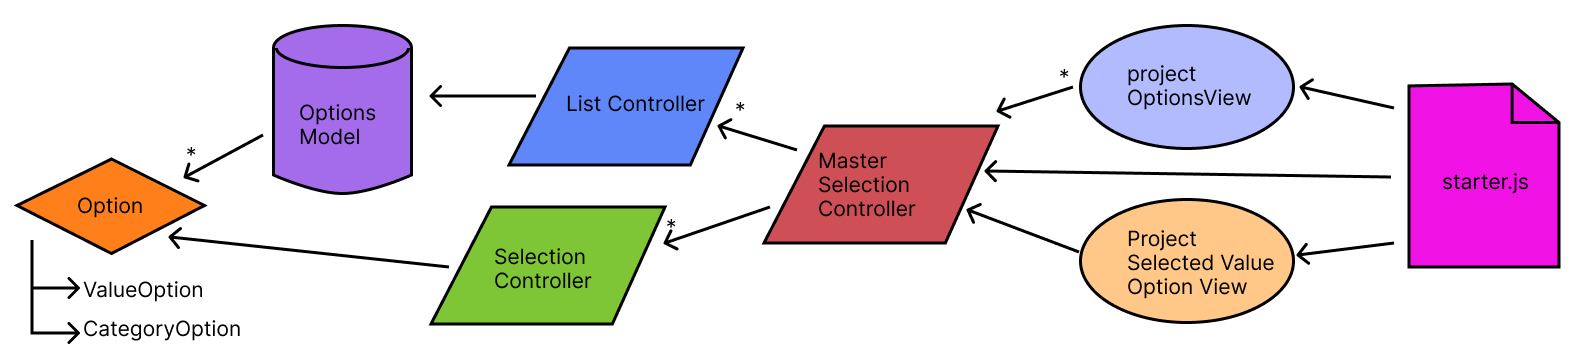
\includegraphics[width=120mm]{diagram-select-component-old.png}
    \caption{\centering Diagramm Select Component – erste Version}
    \label{img:diagramSelectComponentOld}
\end{figure}

Diese Version zeigt noch viel Komplexität und duplizierenden Code in den einzelnen Funktionen. 
Eine genaue Analyse der Komponente zeigt, dass sich das Pattern zwei Mal anwenden lässt. 
Die neue Aufteilung ergibt die zwei folgenden Abbildungen \ref{img:diagramColumnComponent} und \ref{img:diagramSelectComponent}. 
Die Implementation der dargestellten Diagramme resultiert aus einem Refactoring im grösseren Rahmen. 

\begin{figure}[!htb]
    \centering
    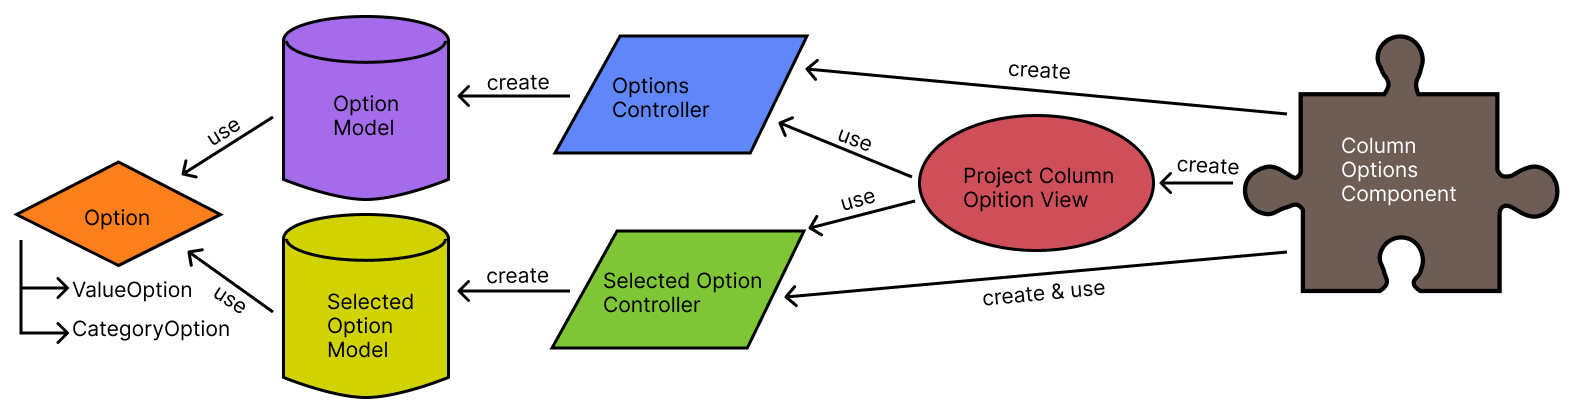
\includegraphics[width=120mm]{diagram-column-component-with-desc.png}
    \caption{\centering Diagramm \codestyle{ColumnOptionsComponent}}
    \label{img:diagramColumnComponent}
\end{figure}

Zum einen findet sich das Projector-Pattern in einer einzelnen Spalte in der Options-Liste wieder. 
Pro Kolonne existieren eine Auswahl und eine Menge von Optionen. 
Diese beiden Bestandteile besitzen je ein eigenes Model und einen eigenen Controller. 
Der Projektor generiert eine gemeinsame View und bindet diese an die beiden Controller. 
Bei einer Anwendung übernimmt die \codestyle{ColumnOptions\-Component} die Verwaltung gewisser Bausteine – mehr dazu später. 

\begin{figure}[!htb]
    \centering
    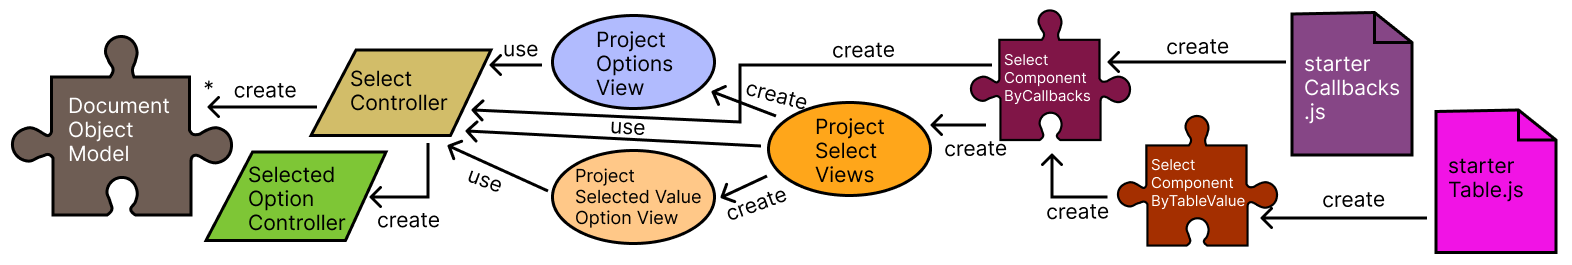
\includegraphics[width=120mm]{diagram-select-component-with-desc.png}
    \caption{\centering Diagramm \codestyle{SelectComponent}}
    \label{img:diagramSelectComponent}
\end{figure}

Die Anwendungskomponente einer Column findet sich als Bestandteil des zweiten Projector-Patterns wieder. 
Ein \codestyle{SelectController} verwaltet eine bis mehrere \codestyle{Column\-Optoions\-Component}s sowie ein Element für die Tastaturnavigation. 
Die sogenannte Cursor-Position verwendet im Hintergrund ebenfalls einen \codestyle{SelectedOptionController}. 
Dieser ist derselbe wie in der Abbildung \ref{img:diagramColumnComponent} und findet hier eine Wiederverwendung. 
Für die Definition der Bindings greifen die einzelnen Projektoren auf denselben Controller zu. 
Der Master-Detail-Aufbau der neuen Komponente findet sich in der Aufteilung der Projektoren wieder. 
Der Detail-Baustein kümmert sich um die aktuelle Auswahl und das Eingabefeld. 
Die Master-Komponente verwaltet alle Spalten mit den Kategorie- und Werte-Optionen sowie deren Bindings. 
Eine weitere Funktion ist die Einbettung der beiden Projektoren in eine gemeinsame View. 
Auch diese Projector-Pattern-Anwendung schliesst mit einer Component – der \codestyle{SelectComponent} – ab. 
Mehr zu dieser und der \codestyle{ColumnOptions\-Component} steht im nächsten Kapitel. 


\subsection{Decorator Pattern}
\label{sec:decoratorPattern}

Ein Decorator\citemarktext{
    [\cite{decoratorPattern}]
} bietet zusätzliches Verhalten, ohne das originale Objekt zu verändern. 
Dabei lassen sich verschiedene Funktionen kombinieren. 
Dieses Pattern ermöglicht die Erstellung eines modularen und anpassbaren Codes. 
In diesem Projekt unterstützt es die Gestaltung und Erweiterung der Auswahlkomponente. 

Wie im vorherigen Kapitel erwähnt, besteht die neue Komponente unter anderem aus zwei sogenannten Component-Bausteinen. 
Die Decorator sind in den Abbildungen \ref{img:diagramColumnComponent} und \ref{img:diagramSelectComponent} als Puzzle dargestellt. 
Diese Bestandteile kombinieren die Funktionalität des Controllers mit der Erstellung der View. 
Dadurch lässt sich die neue Komponente einfacher anwenden. 

\begin{lstlisting}[style = htmlcssjs, caption = \codestyle{SelectComponentByTableValues} dekoriert \codestyle{SelectComponentByCallbacks}, label = code:componentDecorator]
const SelectComponentByTableValues = (
    selectAttributes,
    optionsTable,
    sortColumnOptionsAlphabetical = false
) => {
    /* code for mapping between table and callbacks */
    const component = SelectComponentByCallbacks(selectAttributes, callbacks);
    return {
        ...component,
    };
};
\end{lstlisting}

Ein weiterer Einsatzort ist in der Abbildung \ref{img:diagramSelectComponent} aus dem Vorkapitel zu sehen. 
Der \codestyle{SelectComponentByTableValues} in Code \ref{code:componentDecorator} dekoriert die \codestyle{SelectComponentByCallbacks}. 
Damit bietet die neue Komponente zwei verschiedene Möglichkeiten der Anwendung. 
Das nächste Kapitel geht genauer auf den Master-View-Bereich des \codestyle{SelectProjector}s – Abbildung \ref{img:diagramSelectComponent} – ein. 


\section{Dropdown-Container}
\label{sec:dropdownContainer}

Für die Darstellung aller Optionen (zu gegebener Zeit) stehen verschiedene Varianten zur Auswahl. 
Eine Möglichkeit ist, den Container als HTML-Dialog zu gestalten. 
Die vorhandenen Funktionen sind jedoch nicht für diese Komponente geeignet. 
Für den gewünschten Zweck erfordert das Dialog-Element noch einiges an benutzerdefinierter Anpassung. 

Eine weitere Variante ist, ein normales \codestyle{div} als Options-Container zu verwenden. 
Dies erfordert ebenfalls einen enormen Implementationsaufwand. 
Eine Anwendung dieses Ansatzes findet sich in der ersten Version der Komponente. 
Hierbei eröffnet sich das Problem der Inkonsistenz zwischen UI und Controller. 
Zudem ist es möglich, dass unerwünscht mehrere Dropdown-Container gleichzeitig offen sind. 

Als dritte Möglichkeit bietet sich die Popover-API an. 
Seit 2024 unterstützen alle gängigen Browser diese Schnittstelle. 
Durch das Refactoring der Variante mit dem normalen Div-Container resultiert eine Version mit der Anwendung dieser API. 
Im Gegensatz zu den beiden oben erwähnten Container-Implementationen reduziert sich durch diese Schnittstelle der Zusatzaufwand. 
Der Grundaufbau des Popover-Containers ist im folgenden Code \ref{code:popoverExample} dargestellt. 

\begin{lstlisting}[style = htmlcssjs, caption = Beispiel – Popover-Container, label = code:popoverExample]
<div popover="auto"
     id="select-component-0-options" 
     class="options-component" 
> <!-{}- content -{}-> </div>
\end{lstlisting}

Bei diesem Codeausschnitt (\ref{code:popoverExample}) ist wichtig, dass das Attribut \codestyle{popover} den Wert \codestyle{auto} erhält. 
Dies bewirkt, dass die Popover sich automatisch schliessen, wenn ein Klick ausserhalb des Containers passiert. 
Das Öffnen und Schliessen des Dropdown-Elements lässt sich über das \codestyle{popovertarget}-Attribut auf der Bedienkomponente steuern. 
Dieses Target enthält die \codestyle{id} des Div-Containers mit dem Attribut \codestyle{popover}. 
Als Alternative dazu besteht die Möglichkeit, das Popover über JavaScript zu steuern. 
Hierbei besteht die Möglichkeit, auf den Status und das Event des Togglens zuzugreifen. 
Diese Funktionalitäten erlauben dem Controller, sich konsistent zum UI zu halten. 

Obwohl nur die Unterstützung der aktuellen Browser verlangt ist, soll die Komponente ältere Browser-Versionen nicht komplett ignorieren. 
Erst seit April 2024 unterstützen alle Browser die Popover-API. 
Ein Test auf einem veralteten Firefox zeigt, dass die Komponente wegen der Popover-Funktionalität einen Fehler in die Console wirft.
Dadurch visualisiert der Browser die Komponente nicht. 
Der folgende Code \ref{code:popoverWorkaround} fängt die Fehlermeldung ab. 

\begin{lstlisting}[style = htmlcssjs, caption = Workaround für ältere Browser, label = code:popoverWorkaround]
try {
    /* code block with 
        `popoverContainer.showPopover();`
    or  `popoverContainer.hidePopover();`
    */
} catch (e) {
    /* inform user about unsupported popover 
       the first time an alert popup appears */
}
\end{lstlisting}

Ein Alert-Popup informiert den Nutzer über Einschränkungen (Abbildung \ref{img:msgOldFirefoxNewComp} im Anhang \ref{chap:newImgs}). 
Einige zusätzliche CSS-Definitionen garantieren eine halbwegs ansehnliche Darstellung. 
Veraltete Browser, welche das nested CSS\footnote{
    Verschachtelter CSS-Code mit Verwendung der \codestyle{\&}-Funktionalität
} und das CSS-\codestyle{:has()} nicht unterstützen, zeigen die neue Komponenten inkonsistent an. 


\section{Performance}
\label{sec:performance}

Mit der Kenntnis des Rendering-Prozesses einer Webseite lässt sich eine gute Performance umsetzen. 
Dieser Ablauf ist im Kapitel \textbf{\nameref{chap:background}} unter \textbf{\nameref{sec:structureRendering}} genau beschrieben. 
Die folgende Abbildung \ref{img:renderingProcessRecap} zeigt die Kernelemente des Prozesses nochmals im Überblick. 

\begin{figure}[!htb]
    \centering
    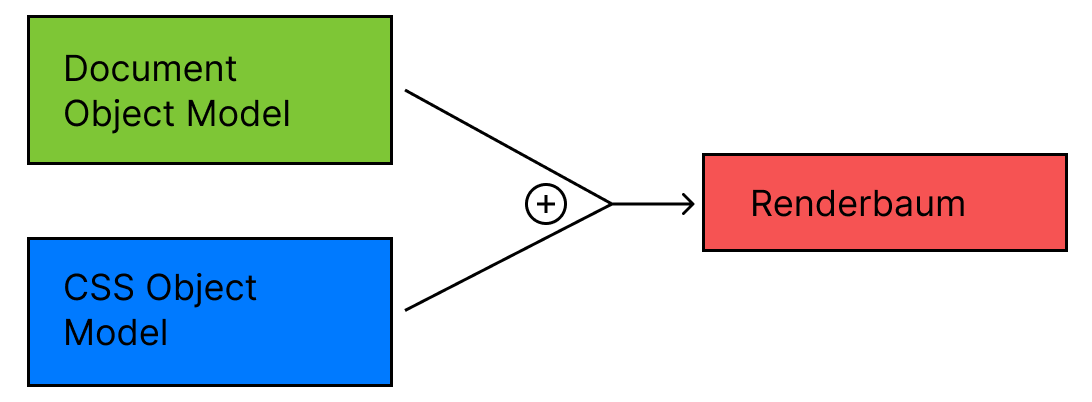
\includegraphics[width=80mm]{rendering-process.png}
    \caption{\centering Rendering-Prozess}
    \label{img:renderingProcessRecap}
\end{figure}

Zur Auffrischung die wichtigsten Punkte nochmals: 
Der Browser kann die Webseite maximal 60 Mal pro Sekunde neu zeichnen. 
Änderungen am DOM (Abbildung \ref{img:renderingProcessRecap}) lösen das Rendern aus. 

Deswegen müssen viele kleine Änderungen ausserhalb des Browser-DOMs\footnote{
    Im Renderbaum verwendeter und im Browser angezeigter DOM
} – am besten in einem sogenannten Shadow-DOM – geschehen. 
Ein Shadow-DOM ist ein Teilbaum, welcher nicht am Browser-DOM angehängt ist. 
Für einen reibungslosen Ablauf ist es sinnvoll, die Änderungen nach dem Abhängen des Elternknotens zu vollziehen. 
Nach den Änderungen ist der Teilbaum wieder an den gewünschten Ort einzuhängen. 

\begin{lstlisting}[style = htmlcssjs, caption = Performance-Optimierung, label = code:performanceOptimization]
const addAllOptions = (options) => {
    const placeHolder = createHolder();
    columnView.replaceWith(placeHolder);
    if (options.length > 50) {
        // same work as else but async
    } else {
        options.forEach((option) => {
            optionsController.addOption(option);
        });
        updateScrollbar(columnView);
        placeHolder.replaceWith(columnView);
    }
};
\end{lstlisting}

Code \ref{code:performanceOptimization} ist eine Stelle, die diese Technik verwendet. 
Das Anzeigen eines Platzhalters mit einem Lade-Indikator an der Ursprungsstelle bewirkt, dass der Nutzer ein Feedback erhält. 
Sobald der Spalten-Container abgekoppelt ist, lädt die Funktion die Optionen in den Shadow-DOM. 
Nach Abschluss ersetzt sich der Lade-Indikator der originalen Stelle im Renderbaum durch den Container mit den neuen Elementen. 

Weiterhin ist darauf zu achten, dass CSS-Klassen\citemarktext{
    [\cite{efficientDomManipulation}]
} an Stelle von Inline-Styles\footnote{
    Offizieller Begriff: Element attached style $\Rightarrow$ Styles direkt im HTML-Element mit Attribut \codestyle{style} definiert
} ihre Verwendung finden. 
Die Selektoren sollten hierarchisch möglichst flach und nicht verschachtelt sein. 
Wenn es die Situation erlaubt, ist es besser, nicht mit \codestyle{innerHTML} zu arbeiten. 
In diesem Projekt ist es für die Anzeige der Label jedoch nötig, \codestyle{innerHTML} zu nutzen. 
Dies liegt daran, dass ein Label auch ein Bild enthalten kann. 
Generell verwendet die neue Auswahlkomponente keine Inline-Styles. 
Die einzige Ausnahme betrifft das verborgene Eingabefeld. 
Durch den Code \ref{code:inlineStyle} sind die Properties vor dem einfachen Überschreiben\footnote{
    \codestyle{!important} nicht verwenden
} geschützt. 

\begin{lstlisting}[style = htmlcssjs, caption = Inline-Style für Input-Feld, label = code:inlineStyle]
inputElement.setAttribute(
    "style", "all:            unset       !important; " +
             "z-index:        -1          !important; " +
             "position:       absolute    !important; " +
             "inset:          5px         !important; " +
             "color:          transparent !important; " +
             "pointer-events: none        !important; "
);
\end{lstlisting}

Die Regeln in Code \ref{code:inlineStyle} sorgen dafür, dass das Input-Feld sowohl transparent als auch resettet ist. 
Zudem befindet es sich im Hintergrund und besitzt dieselbe Grösse wie der Container mit dem ausgewählten Wert. 


\subsection{Performance-Vergleich}
\label{sec:performanceCompare}

Durch die Anpassungen der Performance-Optimierung verschnellert sich die Ladezeit bei grossen Datenmengen enorm. 
Die Testseite enthält vier existierende und vier neue Auswahlkomponenten mit denselben Inhalten wie je eine der existierenden. 
Je eine der Selects enthält eine grosse Datenmenge von über 4'000 Werten. 
Die folgenden zwei Bilder \ref{img:performanceTestBefore} und \ref{img:performanceTestAfter} zeigen die Messung während des Seitenaufbaus. 

\begin{figure}[!htb]
    \centering
    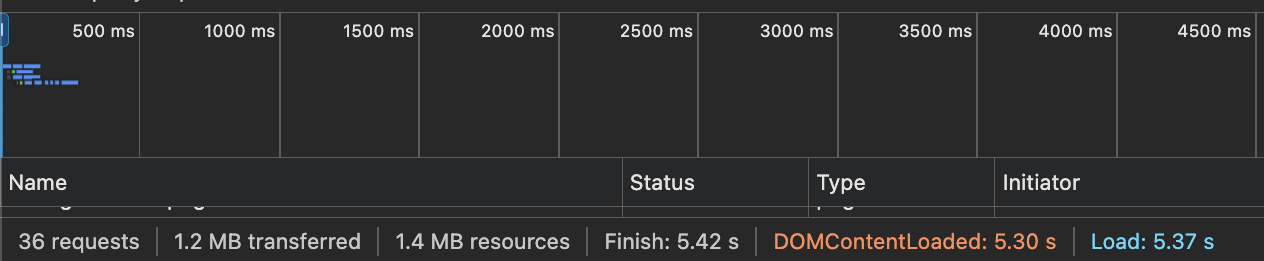
\includegraphics[width=120mm]{performance-before-user-tests-zoom.png}
    \caption{\centering Performance-Test vor Anpassungen}
    \label{img:performanceTestBefore}
\end{figure}

Die Grafik \ref{img:performanceTestBefore} zeigt die mit über 5 Sekunden (rechts unten in Blau) lange Ladedauer der früheren Version. 
Die Implementation führte sehr viele Aktionen auf dem Renderbaum aus. 
Die lange Wartezeit bestätigten mehrere Feedbacks der Nutzer – später mehr dazu. 

\begin{figure}[!htb]
    \centering
    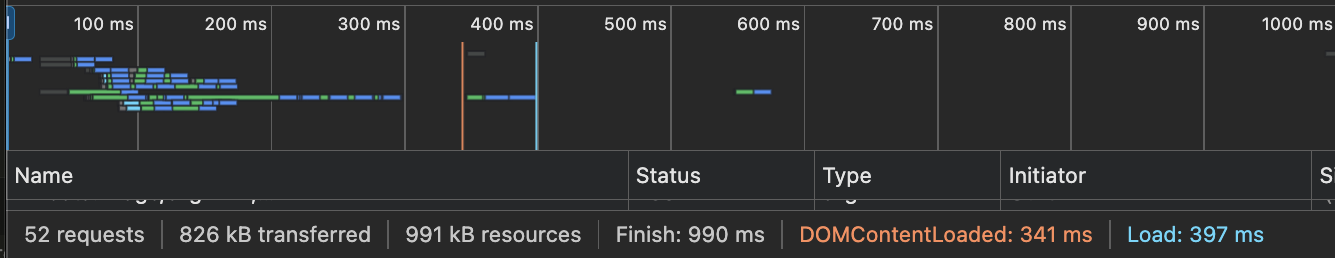
\includegraphics[width=120mm]{performance-after-user-tests-zoom.png}
    \caption{\centering Performance-Test nach Anpassungen}
    \label{img:performanceTestAfter}
\end{figure}

Ein Refactoring der früheren Implementation führt zur Auslagerung der aufwendigen Arbeiten auf den Shadow-DOM. 
Dadurch verkürzt sich der Ladevorgang um vier bis fünf Sekunden auf knapp 0.4 Sekunden (rechts unten in Blau). 
Der Vergleich zwischen Abbildung \ref{img:performanceTestBefore} und \ref{img:performanceTestAfter} zeigt, dass die Seite um Faktor 13 schneller lädt. 
Feedbacks zu den durchgeführten User-Tests mit Programmierern wie auch Endnutzern sowie manuelle Tests sind im nachfolgenden Kapitel aufgeführt. 


\section{Testing}
\label{sec:testing}

Verschiedene Arten von Tests garantieren die Korrektheit der einzelnen Funktionen und Komponenten. 
In manuellen Tests findet die Kontrolle der Konsistenz im UI und der Interaktion statt. 
Die automatisierten Code-Tests stellen sicher, dass das Aufrufen der gebotenen Funktionalität die gewünschten Änderungen ausführt. 
Komponenten, welche für die Erstellung des UI zuständig sind, prüfen sowohl die Existenz von Elementen als auch das Triggern der Events. 
Die User-Tests mit unterschiedlichen Personen gewährleisten eine gute Nutzerzufriedenheit sowie die intuitive Anwendung durch Programmierer. 
Die Auswahl der Nutzer fällt auf eine grosse Vielfalt, damit die Resultate unterschiedliche Sichtweisen einbeziehen. 


\subsection{Manuelle Tests}
\label{sec:manuelTests}

Manuell durchgeführte Tests – in den vier aktuellen Browsern Edge, Chrome, Firefox und Safari – beweisen die Konsistenz der neuen Komponente. 
Als Beispiel dient die \codestyle{SelectComponent} mit drei Spalten (Abbildung \ref{img:manualTestComponentOsx}). 

\begin{figure}[!htb]
    \centering
    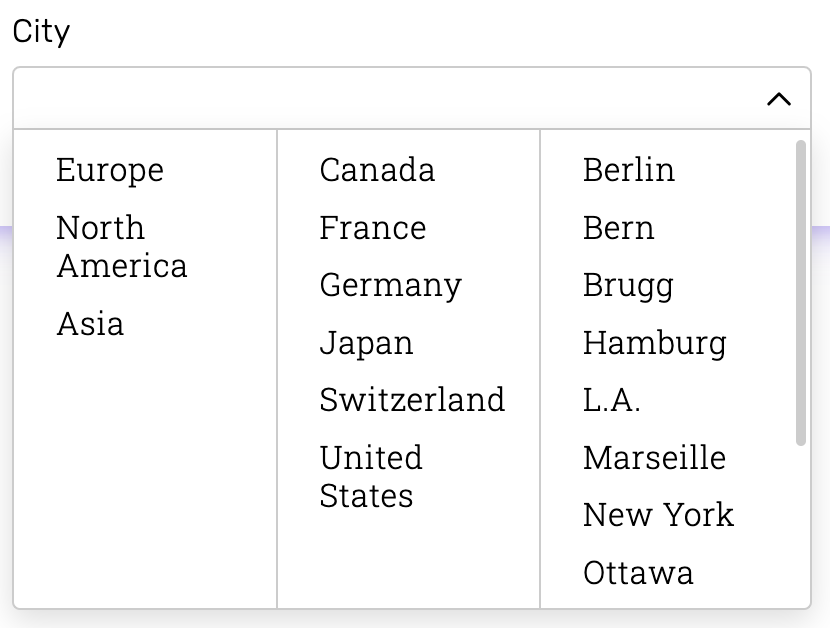
\includegraphics[width=80mm]{newComponent/opened.3col.png}
    \caption{\centering Neue Komponente auf OSX}
    \label{img:manualTestComponentOsx}
\end{figure}

Diese Komponente unterzieht sich sowohl einer Prüfung auf Mac als auch Windows. 
In den Einstellungen sind in einem ersten Durchgang der Light-Mode und in einem Zweiten das Dark-Theme gespeichert. 
Die genaue Kombination zwischen Browsern und Betriebssystemen ist wie folgt: 

\begin{itemize}
    \item \textbf{Mac} bzw. \textbf{OSX}: Chrome (127), Firefox (128), Safari (17.5)
    \item \textbf{Windows (10/11)}: Chrome (127), Firefox (128), Edge (127)
\end{itemize}

Die SelectComponent aus Abbildung \ref{img:manualTestComponentOsx} zeigt sich in den aufgezählten Kombinationen grundlegend konsistent. 
Es existiert nur eine kleine Abweichung. 
Die Scrollbars auf Windows (Abbildung \ref{img:manualTestComponentWin}) besitzen auf der rechten Seite einen grösseren Abstand als auf Mac (Abbildung \ref{img:manualTestComponentOsx}). 

\begin{figure}[!htb]
    \centering
    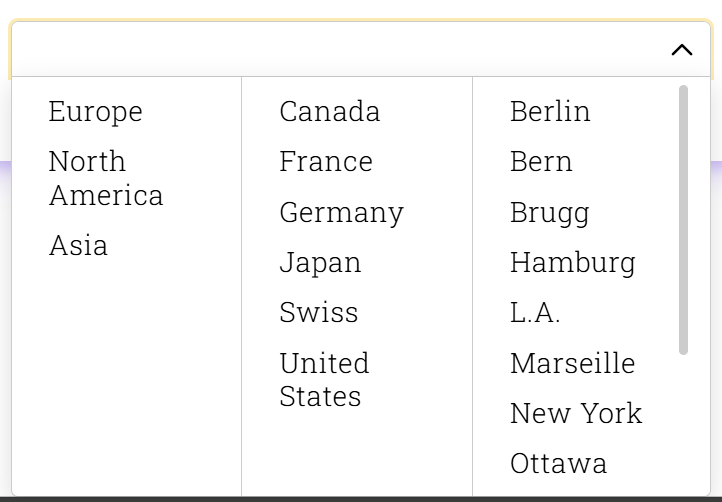
\includegraphics[width=80mm]{newComponent/win.chrome.png}
    \caption{\centering Neue Komponente auf Windows}
    \label{img:manualTestComponentWin}
\end{figure}

Dabei spielt der Browser keine Rolle. 
Bei den Interaktionen verhält sich die Komponente ebenfalls konsistent über alle Browser. 
Die einzige Abweichung findet sich beim Ausführen von Aktionen. 
Auf Windows-PCs mit Nummernpad funktionieren die Page\-Up-, Page\-Down-, Home- und End-Keys\footnote{
    Gewisse Tastaturen besitzen die genannten Tasten doppelt – einmal im Nummernpad und einmal in der obersten Zeile
} auf der Tastatur. 
Auf OSX verlangen die oben genannten Tasten und Delete eine Tastenkombination mit der fn-Taste. 

Zusätzlich zu den im Vorfeld vereinbarten Systemen und Browsern finden noch folgende weitere Prüfungen statt: 

\begin{itemize}
    \item \textbf{Linux (24 LTS)}: Firefox (125), Chromium (127)
    \item \textbf{iOS (Simulator)}: Safari (17.2)
    \item \textbf{Android (Pixel Simulator)}: Chrome (124)
\end{itemize}

Diese Tests beweisen, dass die Komponente über die geforderten Umgebungen hinaus funktioniert. 
Firefox zeigt die \codestyle{SelectComponent} auf Linux wie auf OSX an. 
Speziell die Scrollbar in den Spalten ist rechts anliegend. 
In Chromium besteht ein Abstand von der Scrollbar zum rechten Rand. 
Ansonsten ist die Komponente konsistent im UI und der Interaktion. 

Die mobilen Geräte öffnen keine virtuelle Tastatur. 
Deswegen sind nur Touch-Inter\-aktionen möglich. 
Zu diesen Bedienungsmöglichkeiten gehören das Scrollen und das Klicken. 
Auf iOS und auf Android stellen die Browser das UI meist konsistent – wie auf dem Desktop Safari – dar. 
Die Scrollbar ist anliegend an der rechten Seite. 
Das Highlight und die Cursor-Position haben keinen weiteren Nutzen. 
Die beiden Zustände bewegen sich mit der Selektion mit. 
Das Highlight verschwindet, wenn das Touch ausserhalb einer Option erfolgt. 
Die einzige Inkonsistenz auf iOS zeigt sich beim Klick ausserhalb der \codestyle{SelectComponent}. 
Anders als Safari auf Desktop schliesst diese Interaktion den Container nicht. 
Wenn der Klick auf der X einen bereits selektierten Wert löscht, bleibt der Container ebenfalls offen. 
Auf dem Pixel Chrome reagiert der Klick auf die Detail-Ansicht abweichend. 
Ist das Popover bereits geöffnet, schliesst die Interaktion dieses und öffnet es gleich wieder. 
Trifft die Touch-Geste das X bei einer bereits getroffenen Selektion, passiert dieser Fehler nicht.  

Folgende veraltete Browser finden sich in oberflächlichen Tests wieder: 

\begin{itemize}
    \item \textbf{Mac}: Firefox Version 123 $\Rightarrow$ vor Popover-API
    \item \textbf{iOS}: Safari Version 16.7 $\Rightarrow$ vor Popover-API
\end{itemize}

In veralteten Browsern ist die \codestyle{SelectComponent} mit leichten Einbussen nutzbar. 
Der aufgelistete Firefox und auch Safari öffnen die neue Komponente normal. 
Im offenen Zustand ist das Toggle-Icon dasselbe wie im geschlossenen. 
Ein Klick ausserhalb der Komponente schliesst den Listencontainer nicht. 
Daher existiert die Inkonsistenz, dass mehrere Auswahlkomponenten parallel geöffnet sein können. 
Dies ermöglicht eine unerwünschte Darstellung von überschneidenden Listencontainern. 
Das restliche UI zeigt kaum Abweichungen. 
Die Interaktionen funktionieren alle wie in den aktuellen Browserversionen. 
Gewisse Zustände sind im Controller nicht konsistent mitgeführt. 
Ohne das Popover reagiert das Toggle-Event nicht.

Die breite Abdeckung der manuellen Tests beweist bei den anfangs genannten Browsern eine konsistente Darstellung und Interaktion. 
Zudem sind Nutzer mit leicht veralteten Browsern nur leicht beeinträchtigt. 
Eine gewisse Bedienbarkeit ist möglich. 


\subsection{Automatisierte Tests}
\label{sec:automatedTests}

Tests für Komponenten der \codestyle{SelectComponent} beweisen die Stabilität des Codes. 
Generell befinden sich die einzelnen Komponenten nach Separation of Concern je in einer eigenen Testeinheit. 
Dies garantiert das schnelle Auffinden von Bugs und unerwünschtem Verhalten direkt in einer Komponente. 
Auf der Abbildung \ref{img:automatedTests} ist zu sehen, dass eine breite Palette an Kontrollen stattfindet und sauber durchläuft. 

\begin{figure}[!htb]
    \centering
    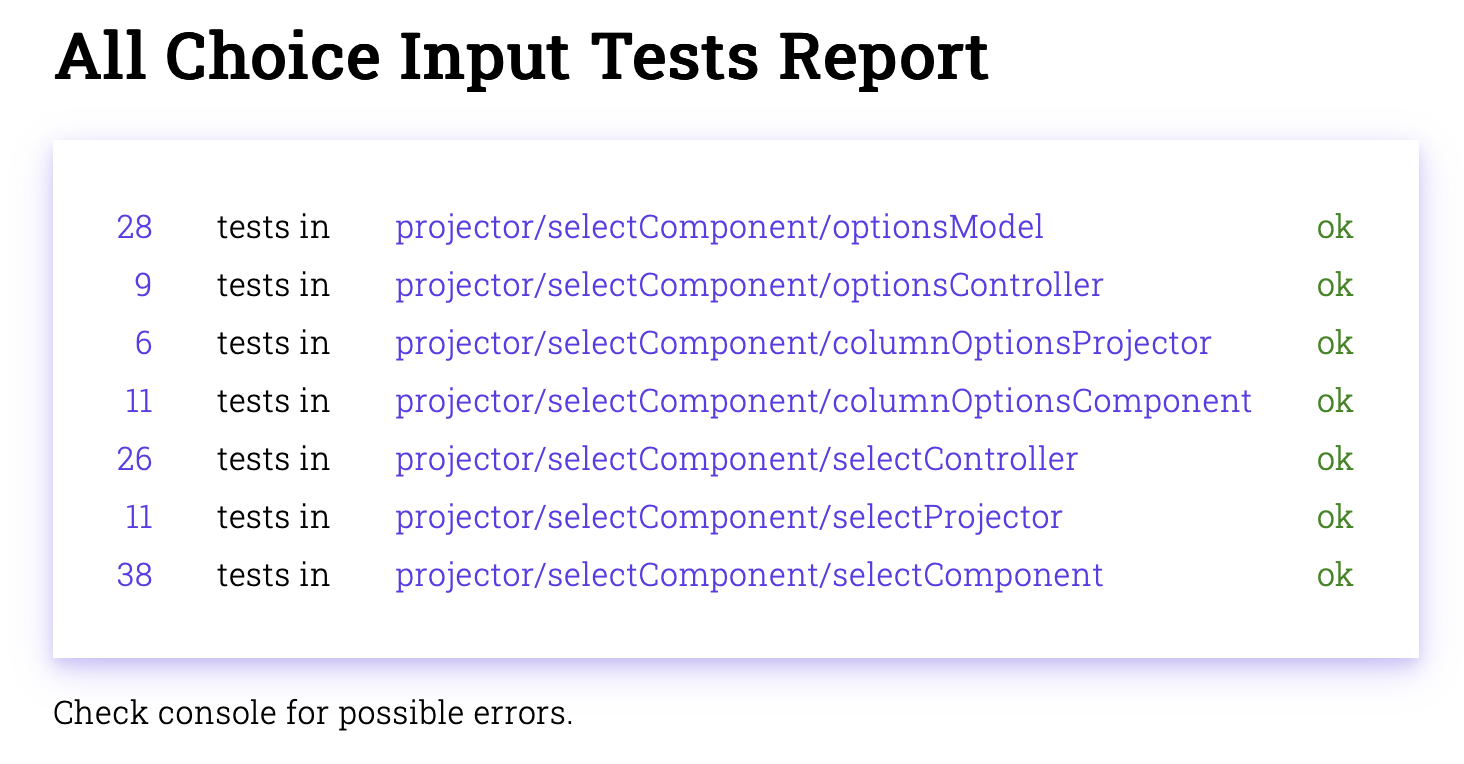
\includegraphics[width=100mm]{automatedTests.png}
    \caption{\centering Automatisierte Tests}
    \label{img:automatedTests}
\end{figure}

Die oberen vier Zeilen auf Abbildung \ref{img:automatedTests} zeigen Tests zu den Bausteinen aus Abbildung \ref{img:diagramColumnComponent}. 
Diese decken den Level der Options bis zur Column ab. 
Die ersten zwei Testsuites kümmern sich genauer um die Korrektheit der Models und Controller. 
Dabei besteht das erste File aus den Tests der Typen \codestyle{ValueOption} und \codestyle{CategoryOption}. 
Dazu gesellen sich Prüfungen der Komponenten \codestyle{OptionsModel} und \codestyle{SelectedOption\-Model}. 
Der \codestyle{Options\-Controller} und der \codestyle{SelectedOption\-Controller} finden sich in der Test-Datei wieder. 
Der \codestyle{project\-ColumnOptions\-View}-Test deckt die Kontrolle des Bindings und die Existenz der View-Elemente ab. 
Die Korrektheit des Zusammenspiels zwischen Projektor und Controller findet sich im \codestyle{Column\-Options\-Component}-Testing wieder. 

Die restlichen Testbibliotheken decken die Korrektheit der auf Abbildung \ref{img:diagramSelectComponent} sichtbaren Bausteine ab. 
Diese drei Dateien prüfen das Zusammenspiel der Columns sowie der allgemeinen Komponentenfunktionalitäten. 
In einzelnen Units prüft die \codestyle{Select\-Controller}-Test-Suite verschiedene Varianten der Anwendung. 
Im \codestyle{project\-Select\-Views}-Test befinden sich – wie bereits bei der Column – die Prüfungen der Korrektheit der View-Elemente und Bindings. 
Die letzte Datei kümmert sich um die Kontrolle der \codestyle{Select\-Component\-By\-Callbacks} und \codestyle{Select\-Component\-By\-TableValues}. 
Die breite Abdeckung der Einzelteile garantiert die korrekte Funktion der neuen Komponente. 
Die Tests im nachfolgenden Kapitel sind sowohl für eine gute Anwendbarkeit im Code als auch für eine angenehme Benutzung der Auswahlkomponente im Browser notwendig. 


\subsection{User-Tests}
\label{sec:userTests}

Die Bewertung des Designs und der Benutzerfreundlichkeit ist ein wichtiger Bestandteil der Entwicklung. 
Die im Vorfeld definierten Personas – Anhang \textbf{\ref{chap:perosnas}} – finden sich in den getesteten Usern wieder. 
Estrid Miller arbeitet als Webentwicklerin und stört sich an schlechter Code-Dokumentation. 
Sie wünscht sich eine flexible und anpassbare UI-Komponente, welche ihre tägliche Arbeit vereinfacht. 
Der Alltagsnutzer Love Berg ist ein typischer Webanwender und ärgert sich über umständliche und langsame Anwendungen. 
Er wünscht sich ein effizientes und verständliches User-Interface. 
Die folgenden zwei Unterkapitel decken mit den zwei Nutzergruppen Programmierer und Endanwender die Personas ab. 


\subsubsection{\color{dblue} Programmierer}
\label{sec:userTestsProgrammer}

Die Probanden dieser User-Tests sind alle Studenten der FHNW. 
Deswegen haben die Testpersonen ein ähnliches Hintergrundwissen wie Estrid. 
Die Vorlieben der Probanden sind unterschiedlich und decken dadurch die Vorgaben durch die Persona ab. 

Im Rahmen der Evaluierung der neuen Dropdown-Komponente sind Programmierer dazu eingeladen, spezifische Aufgaben zu erfüllen. 
Diese Aufgaben umfassen die Implementierung der Dropdown-Komponente in eine bestehende Webanwendung. 
Für den Erhalt eines möglichst realistischen Feedbacks sind die Teilnehmer gebeten, nach der Implementierung eine Google-Umfrage auszufüllen. 

\begin{figure}[!htb]
    \centering
    \begin{minipage}[b]{0.45\textwidth}
        \centering
        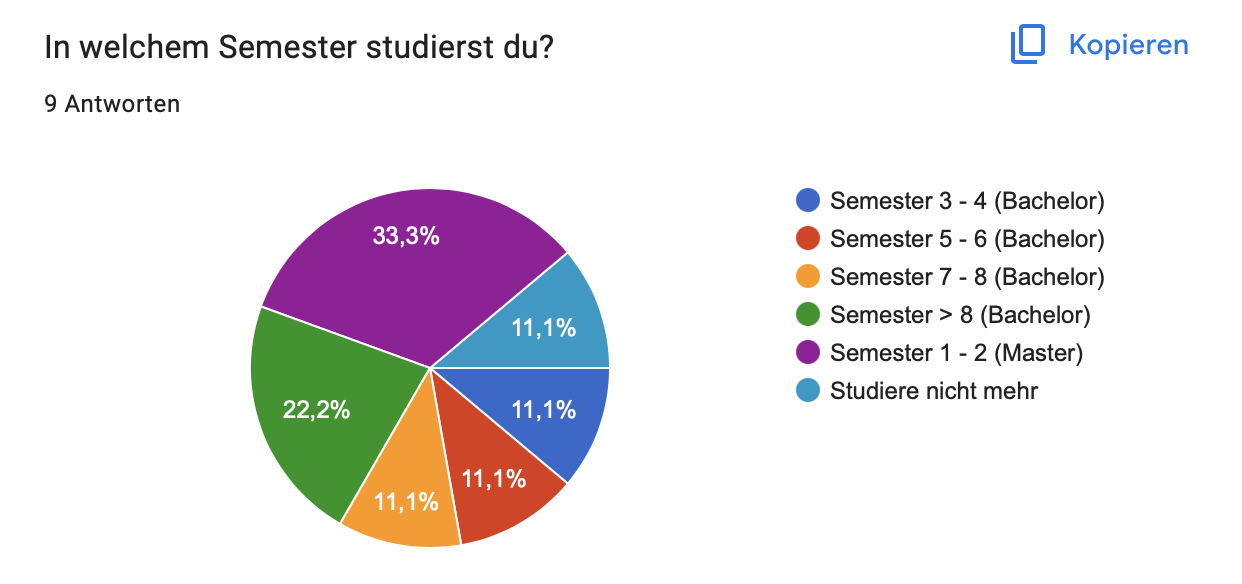
\includegraphics[width=\textwidth]{userTests/semester9.png}
        \caption{\centering Aufteilung Semester}
        \label{img:userTestsSemester}
    \end{minipage}
    \hfill
    \begin{minipage}[b]{0.45\textwidth}
        \centering
        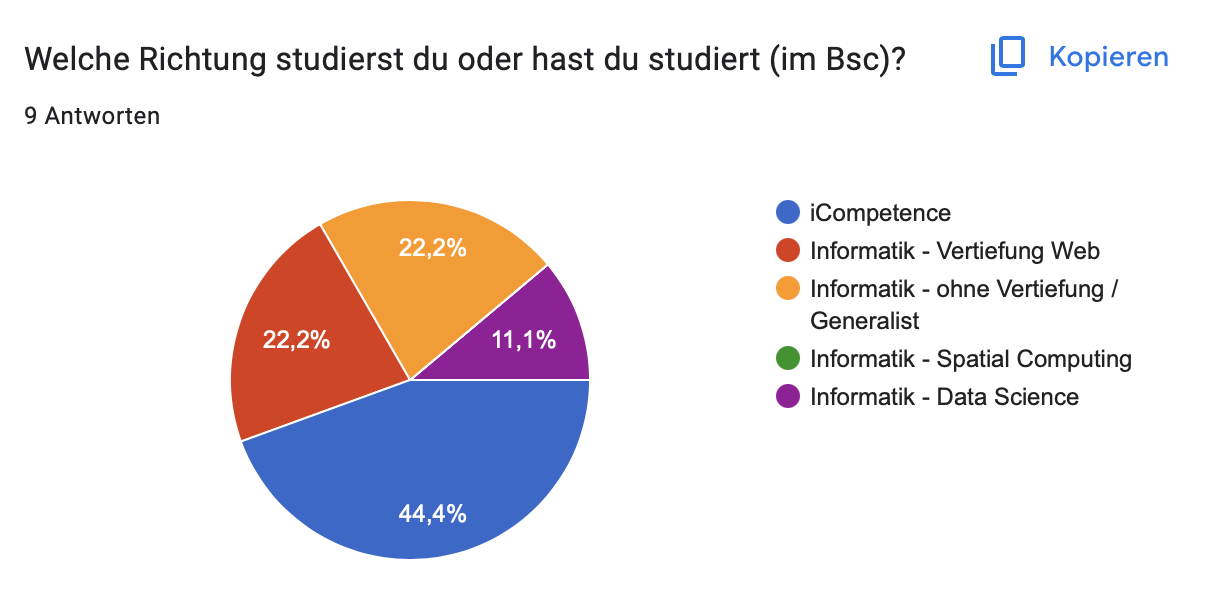
\includegraphics[width=\textwidth]{userTests/richtung9.png}
        \caption{\centering Aufteilung Studienrichtung}
        \label{img:userTestsStudy}
    \end{minipage}
\end{figure}

Insgesamt haben 9 Studenten an dem User-Test teilgenommen und die Aufgaben versucht zu lösen. 
Die Grafiken \ref{img:userTestsSemester} und \ref{img:userTestsStudy} zeigen, dass die Hintergründe der Probanden breit gefächert sind. 
Zwei der Testpersonen konnten die Aufgabe nicht korrekt lösen. 

Die Aufgaben beinhalten verschiedene Szenarien. 
Die Entwickler sollen die neue Komponente unter anderem für das Mittagessen, eine Heimatregion oder ein Geburtsjahr einsetzen. 
Der bereitgestellte Code (Anhang \ref{chap:userTestProgrammers}) dient als Basis für die Implementierung. 
Dabei fällt der Fokus darauf, dass die Programmierer die Anbindung an die vorhandene Infrastruktur korrekt umsetzen. 

Nach der systematischen Erfassung der Umfrage-Rückmeldungen erfolgt das Analysieren dieser. 
Programmierer bewerten die Komponente als benutzerfreundlich und ästhetisch ansprechend. 

\begin{figure}[!htb]
    \centering
    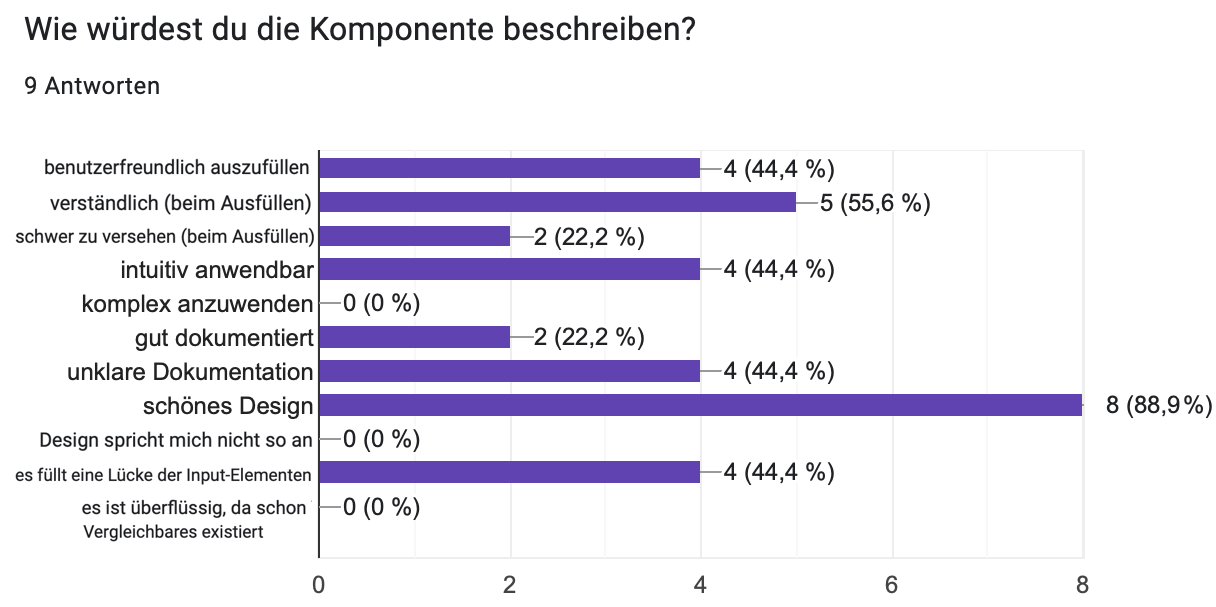
\includegraphics[width=100mm]{userTests/desc9.png}
    \caption{\centering Meinungen der Testpersonen}
    \label{img:userTestsDescription}
\end{figure}

Die Umfrageergebnisse zeigen eine überwiegend positive Bewertung der Komponente (Abbildung \ref{img:userTestsDescription}). 
Sie sind in den Abbildungen \ref{img:userTestSemester} bis \ref{img:userTestUsage} im Anhang \ref{chap:userTestProgrammers} illustriert. 
Einige Teilnehmer äussern jedoch Kritikpunkte hinsichtlich der Dokumentation. 
Insbesondere die Beschreibung der Rückgabewerte und die Integration von Callbacks wiesen vor der Anpassung Schwierigkeiten auf. 
Weitere Verbesserungsvorschläge umfassen die Möglichkeit, die Komponente nach der Auswahl automatisch zu schliessen. 

Personen mit nur geringen JavaScript-Kenntnissen fällt es schwer, die Komponente intuitiv zu verwenden. 
Die Testperson ohne jegliche JavaScript-Kenntnisse konnte die Aufgaben nicht korrekt lösen. 
Für einige Testnutzer ist die Verwendung von Callbacks als Service-Funktionen eine Stolperfalle. 

Die Ergebnisse der Tests liefern wertvolle Erkenntnisse, welche zur Verbesserung der Dokumentation beitragen. 
Die Überarbeitung der Dokumentation wie auch die der Rückgabe der Komponente heben die Kritik auf. 
Die Erstellung des zweiten Konstruktors mit einer Tabelle von Werten ermöglicht das Umgehen des Stolpersteins der Callbacks. 

Die nachfolgende Liste zählt die Verbesserungsvorschläge und Bemerkungen der Testprogrammierer zusammengefasst auf. 
Die genauen Feedbacks befinden sich im Anhang \textbf{\ref{chap:userTestProgrammers}}. 
 \\
\textbf{Dokumentation \& Return-Wert}: 
Das JSDoc von \codestyle{SelectComponent} benötigt eine detailliertere Beschreibung des Return-Arrays. 
Die Elemente erklären sich erst in den Anwendungsbeispielen. 
Tester mussten nach der Beschreibung suchen. 
Die Dokumentation erweist sich als verwirrend. 
Wenn sich die Komponente nicht im Projektordner befindet, erscheinen keine Typen-Informationen bzw. Dokumentationshinweise. 
\\
\codestyle{\textbf{numberOfColumns}}: 
Ein Tester versuchte den Parameter falsch anzuwenden, um Fehler aufzudecken. 
Ist \codestyle{selectAttributes} $\Rightarrow$ \codestyle{numberOfColumns} nötig? 
\\
\codestyle{\textbf{selectAttributes}}: 
Der Parameter ist intuitiv anwendbar. 
Label, Name und \codestyle{numberOf\-Columns} sind klar. 
\\
\textbf{Callback}: 
Der Parameter ist nicht intuitiv anwendbar. 
Callbacks sind nicht allen Programmierern klar in der Anwendung bzw. bekannt. 
Es ist speziell, dass – im Gegensatz zum UI – das \codestyle{serviceCallbacks}-Array in umgekehrter Reihenfolge einzugeben ist. 
\\
\textbf{Navigation}: 
Die Tastaturnavigation ist nicht ideal. 
Die Verwendung der Tastatur zum Eingrenzen möglicher Kategorien/Werte – unscharfe Suche\footnote{
    Elemente durch das Übereinstimmen von Zeichen oder einer Zeichenkette finden.
} – wäre eine Möglichkeit. 
Sonst dauert die Suche länger als in den existierenden Komponenten. 
\\
\textbf{Automatisches Schliessen}: 
Automatisches Schliessen der Komponente nach der Auswahl wäre praktisch. 
\\
\textbf{Performance}: 
Die Performance ist zu langsam. 
Beim Implementieren von Task 2.2 benötigt die Webseite ca. 5 Sekunden zum Laden. 
Dies liegt – soweit ersichtlich – am HTML-Rendering. 
\\
\textbf{Leere Spalten}: 
Wenn zwei Kolonnen sichtbar sind, aber rechts nichts selektierbar ist. 
Das ist ein zu erwartender Fall, aber nicht ideal für die Demo. 


\subsubsection{\color{dblue} Endanwender}
\label{sec:userTestsEnduser}

Im Rahmen der Usability-Tests erfolgt eine Untersuchung der Benutzerfreundlichkeit der neuen Dropdown-Komponente.  
Die Komponente nutzt eine mehrstufige Filterung. 
Dies erleichtert die Navigation innerhalb langer Listen. 
Die Probanden durchlaufen zwei Aufgaben. 
Diese zielen auf die Evaluation der Effizienz und Anwenderfreundlichkeit dieser Dropdown-Funktion ab. 

 \\
\emph{Aufgabenbeschreibung}: 

\begin{itemize}
    \item[1.] \textbf{Jahresauswahl}: 
              Testpersonen wählen das gewünschte Jahr aus einer Liste aus. 
              Der Prozess beinhaltet die Vorauswahl eines Jahrzehnts, gefolgt von der Auswahl des spezifischen Jahres. 
              Diese Aufgabe dient der Bewertung der Benutzerfreundlichkeit und Effizienz der Filteroption. 
    \item[2.] \textbf{Stadtauswahl}: 
              Die Testpersonen wählen eine spezifische Stadt aus einer dreispaltigen Dropdown-Liste. 
              Die Auswahl erfolgt schrittweise: Beginnend mit dem Kontinent, gefolgt vom Land und schliesslich der Stadt. 
              Der Fokus liegt hierbei auf der Bedienbarkeit und der Wirksamkeit der Filterfunktion. 
\end{itemize}

 \\
\emph{Feedback der Testpersonen}: 

\begin{itemize}
    \item Allgemeine Benutzerfreundlichkeit: 
    \begin{itemize}
        \item \textbf{Robert (Junger Alltagsbenutzer, Digital Native)}: 
              Empfindet die Drop\-down-Menü\-führung als intuitiv und zügig bedienbar. 
              Sowohl das Jahr als auch die Stadt lassen sich mühelos finden. 
        \item \textbf{Sara (Semi-aufmerksam, nicht so schnell auf der Tastatur)}: 
              Beginnt mit Schwierigkeiten in der Dreispaltenansicht. 
              Nach kurzer Einarbeitung findet sie die Filteroptionen jedoch nützlich. 
        \item \textbf{Nick (Alltagsbenutzer/Student)}: 
              Zeigt sich zufrieden mit der Handhabung. 
              Er hebt hervor, dass die Filterfunktion das Auffinden des Jahres beschleunigt. 
        \item \textbf{Reto (Unternehmer, über 60 Jahre alt)}: 
              Erlebt die Menüführung als etwas komplex, besonders die dreispaltige Filterung. 
              Nach einer Eingewöhnungszeit erkennt er jedoch die Vorteile gegenüber einer langen Liste. 
    \end{itemize}
    \item Funktionalität der Filteroptionen: 
    \begin{itemize}
        \item \textbf{Robert}: 
              Schätzt die Filteroptionen als sehr nützlich ein. 
              Das Finden spezifischer Jahre und Städte gelingt schneller als erwartet. 
        \item \textbf{Sara}: 
              Nutzt zuerst nicht alle Filter bei der Stadtauswahl. 
              Somit scrollt sie ein bisschen mehr. 
        \item \textbf{Nick}: 
              Die Möglichkeit, zuerst das Jahrzehnt und anschliessend das spezifische Jahr auszuwählen, beschleunigt den Prozess erheblich. 
        \item \textbf{Reto}: 
              Ist unsicher bei der Nutzung der Filter. 
              Nach einiger Zeit erkennt er jedoch dessen Vorteil. 
    \end{itemize}
\end{itemize}

 \\
\emph{Visuelle Gestaltung und Übersichtlichkeit}: 

\begin{itemize}
    \item \textbf{Robert}: 
          Beurteilt das Design als klar und ansprechend. 
          Die Struktur erscheint ihm logisch und nachvollziehbar. 
    \item \textbf{Sara}: 
          Findet die visuelle Gestaltung in Ordnung. 
          Sie vermisst jedoch eine deutlichere Hervorhebung aktiver Filteroptionen. 
    \item \textbf{Nick}: 
          Ist zufrieden mit der Übersichtlichkeit und der klaren Struktur des Drop\-down-Menüs. 
    \item \textbf{Reto}: 
          Besonders in der Dreispaltenansicht findet er das Design zunächst verwirrend. 
          Er gewöhnt sich aber daran. 
\end{itemize}

 \\
\emph{Intuitivität der Bedienung}: 

\begin{itemize}
    \item \textbf{Robert}: 
          Erlebt die Bedienung als sehr intuitiv und benötigt keine weiteren Erklärungen. 
    \item \textbf{Sara}: 
          Muss sich an die Bedienung gewöhnen. 
          Jedoch nach kurzer Zeit findet sie die Handhabung einfach. 
    \item \textbf{Nick}: 
          Empfindet die Bedienung als leicht nachvollziehbar und intuitiv. 
    \item \textbf{Reto}: 
          Hat anfänglich Schwierigkeiten und wünscht sich eine einfache Einführung. 
\end{itemize}

 \\
\emph{Gesamtzufriedenheit}: 

\begin{itemize}
    \item \textbf{Robert}: 
          {\color{editorGreen} 10/10} – Sehr zufrieden, bewertet die Filteroptionen als hervorragend. 
    \item \textbf{Sara}: 
          {\color{editorGreen} 7/10} – Zufrieden, dreispaltige Navigation ist ihr jedoch nicht so gängig. 
    \item \textbf{Nick}: 
          {\color{editorGreen} 9/10} – Zufrieden, bevorzugt diese Art der Auswahl. 
    \item \textbf{Reto}: 
          {\color{editorGreen} 8/10} – Zufrieden, jedoch mit anfänglichen Schwierigkeiten. 
          Mag speziell die schnelle Jahresauswahl. 
\end{itemize}

 \\
\emph{Verbesserungsvorschläge}: 

\begin{itemize}
    \item \textbf{Robert}: 
          Hat keine weiteren Vorschläge. 
    \item \textbf{Sara}: 
          Findet die Dreispaltige zwar nützlich. 
          Aber leider müssen mehrere Spalten bearbeitet werden. 
    \item \textbf{Nick}: 
          Schlägt eine kurze Anleitung oder Hinweistext für Erstnutzer vor. 
    \item \textbf{Reto}: 
          Eventuell eine vereinfachte Variante mit weniger Informationen bei der Länderauswahl. 
\end{itemize}

Der Usability-Test zeigt, dass die neue Dropdown-Komponente insgesamt beliebt ist. 
Besonders die Filteroptionen nach Jahrzehnten und Kontinenten erweisen sich als hilfreich. 
Einige Nutzer benötigen jedoch eine Eingewöhnungszeit, um sich an die Bedienung der mehrstufigen Auswahl zu gewöhnen. 


\subsubsection{\color{dblue} Fazit}
\label{sec:userTestsSummery}

Die Entwicklung und Implementierung der neuen Auswahlkomponente stellen eine Herausforderung dar. 
Dies ist durch eine strukturierte Vorgehensweise und kontinuierliche Verbesserungen erfolgreich umsetzbar. 
Die Usability-Tests mit Programmierern und Endanwendern liefern Einblicke in die Benutzerfreundlichkeit und Funktionalität der Komponente. 

 \\
\noindent
\emph{Wichtige Erkenntnisse und Erfolge}: 
\\
\textbf{Design und Konsistenz}: 
Die Nutzung des Kolibri-Designsystems ermöglicht eine konsistente und ansprechende Benutzererfahrung. 
Es ist wichtig, die Farbauswahl und den Kontrast anzupassen. 
Damit sind eine hohe Lesbarkeit sowie auch die Benutzerfreundlichkeit gewährleistet.
\\
\textbf{Interaktion und Benutzerfreundlichkeit}: 
Die neue Komponente bietet eine intuitive Bedienung sowohl für Maus- als auch für Tastaturbenutzer. 
Die Rückmeldungen aus den Tests zeigen, dass die Komponente nach einer kurzen Einarbeitungszeit gut verständlich und benutzerfreundlich ist. 
\\
\textbf{Performance-Optimierungen}: 
Durch gezielte Performance-Optimierungen – wie die Verwendung des Shadow-DOMs – reduziert sich die Ladezeit bei grossen Datenmengen erheblich. 
Dies trägt zu einer flüssigeren Benutzererfahrung bei. 

 \\
\noindent
\emph{Verbesserungspotenziale}: 
\\
\textbf{Dokumentation}: 
Eine detailliertere Dokumentation der Rückgabewerte und der Verwendung der Komponente ist notwendig. 
Die Ausarbeitung des JSDoc vermeidet Missverständnisse und erleichtert die Einarbeitung. 
Dazu unterstützt eine Umgestaltung des Return-Werts die Verständlichkeit der Elemente. 
\\
\textbf{Interaktion}: 
Die Implementierung einer automatischen Schliessfunktion nach der Auswahl eines Wertes ist als wünschenswert identifiziert. 
Eine verbesserte Tastaturnavigation ist ebenfalls erwünscht und findet in der verbesserten Implementation ihren Platz. 
\\
\textbf{Code-Komplexität}: 
Die Reduzierung der Komplexität der Parameter vereinfacht die Komponente in der Verwendung. 
Die daraus resultierende Version der Komponente erhöht durch einen alternativen Konstruktor die Entwicklerfreundlichkeit. 

Die neue Auswahlkomponente erfüllt die Anforderungen an Konsistenz, Benutzerfreundlichkeit und Performance. 
Sie bietet gleichzeitig Raum für weitere Optimierungen. 
Gewisse Kritiken finden ihre Lösung in der neuen Version der Komponente. 
Die \codestyle{SelectComponent} erfüllt durch die kontinuierliche Weiterentwicklung und Verbesserung die hohen Ansprüche moderner Webanwendungen. 


\section{Fazit der neuen Komponente}
\label{sec:summeryNew}

Das Design der Komponente – inspiriert durch das Kolibri-Designsystem – stellt sicher, dass die visuelle Konsistenz und Benutzerfreundlichkeit erhalten bleiben. 
Die spezifischen Designoptionen wie Farbpalette und Layout sind sorgfältig ausgewählt und implementiert. 
Dadurch sind eine optimale Lesbarkeit und Bedienbarkeit gewährleistet. 
Diese Punkte sind durch die durchgeführten Tests bewiesen. 

Der Einsatz von Figma-Prototypen ist entscheidend. 
Daraus erfolgen eine realitätsnahe Vorschau und Benutzerfeedback. 
Aus diesen Gründen verbessert sich die Benutzerfreundlichkeit kontinuierlich. 
Die Kombination von durchdachten CSS-Anpassungen stellt sicher, dass die Komponente intuitiv bedienbar ist. 
Eine klare Interaktionsdefinition garantiert sowohl für Maus- als auch für Tastaturbenutzer eine gute Zugänglichkeit. 

Die Integration von Prinzipien und Patterns führt zu einem stabilen und wartbaren Code. 
Mit KISS und Separation of Concern bleibt der Code einfach und gut lesbar. 
Die Umsetzung vom Null-Object und Projector Pattern garantiert die Wiederverwendbarkeit. 
Diese Patterns halten sich an das Separation of Concern-Prinzip. 
Ein wichtiger Baustein der \codestyle{SelectComponent} ist der Container mit allen Werten. 
Die Wahl der Popover-API vereinfacht die Implementation enorm, da weniger zusätzliche Funktionalität notwendig ist. 

Stetig durchgeführte, manuelle Tests ermöglichen eine Überwachung und einen Vergleich der Performance. 
Optimierungen im Code führen zu einer schnelleren Performance und einer angenehmen Benutzererfahrung. 
Automatische Tests gewährleisten eine hohe Codequalität und die Korrektheit der Funktionalitäten. 
Die durchgeführten User-Tests bestätigten die hohe Usability der Komponente. 
Ein agiles Entwicklungsverfahren ermöglicht während der Entstehung der neuen, effizienten Auswahlkomponente eine stetige Optimierung. 
Die \codestyle{SelectComponent} bildet eine solide Grundlage für zukünftige Erweiterungen und Anpassungen. 
